\documentclass{TeFlon}
\begin{document}
\incorporarDatos{si}{UCM}{Informática}{Desarrollo de Videojuegos}{Tutor:\\ Pedro Pablo Gómez Martín}{2019--2020}{Madrid}{Sergio Gavilán Fernández, Javier Cordero Calvo}{Implementación de realidad mixta para sistema de búsqueda de rutas en dispositivos móviles}
\tnr{no}

%%%%%%%%%%%%%%%%%%%%%%%%%%%%%%%%%%%%%%%%%%% Parte 1 - TFG
\tituloTFG


%\newpage
\chapter*{Autorización de difusión y uso}


%\newpage
\chapter*{Agradecimientos}
\noindent

\indiceTFG
%%%%%%%%%%%%%%%%%%%%%%%%%%%%%%%%%%%%%%%%%%%
%%%%%%%%%%%%%%%%%%%%%%%%%%%%%%%%%%%%%%%%%%% Parte 2



% - Resumenes
\parindent=0em
\section*{Resumen}
\noindent

En este capítulo se ha tratado la integración de ARCore en Unity. Esta integración es necesaria para las aplicaciones de prueba que se han desarrollado utilizando la nube de puntos de ARCore. Del mismo modo, se ha explicado el funcionamiento a fondo de dicha nube de puntos para poder ser utilizada en las aplicaciones de prueba.\\

Por otra parte, una vez que se ha comprendido el funcionamiento de la nube de puntos, se pueden distinguir dos tipos de \textit{shaders}, el de profundidad y el de oclusión. Ambos \textit{shaders} buscan utilizar la nube de puntos de algún modo para generar un efecto de oclusión.\\

Por último, se han estudiado distintas pruebas con dicha nube de cara a medir la eficiencia y la precisión del efecto de oclusión generado con uno de los \textit{shaders}.\\

En el próximo capítulo se profundizará en el funcionamiento de distintas tecnologías de sistema de búsqueda de rutas y de cómo se pueden relacionar con ARCore. Este capítulo se ha visto afectado en contenido por la pandemia del coronavirus o COVID-19. Esta pandemia ha disminuido considerablemente el desarrollo de aplicaciones y pruebas relacionadas con la búsqueda de rutas.
\newpage
\chapter*{Summary}
\addcontentsline{toc}{chapter}{Summary}
\parindent=0em

%Aqui el texto de resumen en INGLES
Summary of TRABAJO DEL FIN DEL GRADO 



%%%%%%%%%%%%%%%%%%%%%%%%%%%%%%%%%%%%%%%%


\section*{Keywords}
\addcontentsline{toc}{section}{Keywords}

%Aqui van las palabras clave en INGLES
English key words


%%%%%%%%%%%%%%%%%%%%%%%%%%%%%%%%%%%%%%%%

% - Capítulos
\parindent=0em
\chapter{Introducción}
\noindent

\parindent=0em
\section{Antecedentes}
\noindent

Antecedentes jejejieji


















\parindent=0em
\section{Objetivos}
\noindent

Los objetivos











\parindent=0em
\section{Plan de trabajo}
\noindent

El plan de trabajo

























\parindent=0em
\chapter{Introduction}
\noindent

\parindent=0em
\section{Antecedents}
\noindent

Antecedentes jejejieji


















\parindent=0em

\section{Goals}
\noindent

The main goal will be to study techniques of occlusion in real time using mobile phones to create a mixed reality environment. Afterwards, that mixed reality environment will be used to create a routes navigation system where there will be virtual objects placed on it to lead the user through the route.\\

That main goal will be divided into the following parts:

\begin{enumerate}[label=\arabic*)]
    \item Develop an occlusion effect in real time for mobile phones.
    
    \item Use that occlusion effect to create an environment of mixed reality.
    
    \item Manage a routes navigation system from a point A to a point B.
    
    \item Navigation of the route through mixed reality elements.
    
\end{enumerate}











\parindent=0em
\section{Work plan}
\noindent

Planning can be divided into two main blocks: occlusion effect on mobile phones and routes search. \\

First of all, in this first part, it should be investigated how ARCore works to obtain information about the depth of objects in the physical world in real time using a single monocular camera. \\

After knowing this information, an investigation will be carried out by reading books and articles on mixed reality to learn more about occlusion. It is important that this knowledge is focused on mobile phones which do not use other cameras than a single monocular camera, as mentioned above. \\

To test the knowledge obtained previously, in this part 3 applications will be implemented:


\begin{itemize}
    \item \textbf{Depth shader application:} It will de developed an application to create a depth map (section~\ref{sec:oclusion}).
    
    \item \textbf{Occlusion shader application:} Application to test efectivity and precision of occlusion shader (section~\ref{shaderOclusionSec}).
    
    \item \textbf{Points cloud application:} This application will be used to test efectivity of the occlusion shader through a points cloud(section~\ref{sec:nubeDePuntos}).
\end{itemize}

With these three applications, the accuracy in generating an occlusion effect in different ways will be checked to keep the most accurate and most efficient one. \\

In the second part, it will be found out what functions the Mapbox search system provides using Unity. Once such information has been obtained, the objective will be to develop an application to test these functionalities. \\

This application will be implemented to obtain GPS coordinates and transform that latitude and longitude into Unity coordinates. Once this is done, the position obtained in Unity will be transformed to a position in the ARCore environment. All this will be done with the final objective of being able to place a virtual object given exact latitude and longitude coordinates.



























\parindent=0em
\chapter{Realidad aumentada, realidad mixta y realidad virtual}
\label{cap:ar_mr_vr}
\noindent

En este capítulo se describen las tecnologías de realidad aumentada, realidad mixta y realidad virtual, además, se habla sobre su uso y los dispositivos necesarios para utilizarlas.

\parindent=0em
\section{Definición}
\noindent

%\footnote{https://www.apple.com/augmented-reality/}

Para poder comprender la tecnología de realidad mixta es necesario conocer los conceptos de realidad aumentada y realidad virtual. La realidad aumentada~\cite{ardefinition} es una tecnología mediante la cual el usuario visualiza el mundo real con el añadido de que puede ver objetos ``sobreimpresionados'', es decir, elementos superpuestos al mundo real.(figura~\ref{fig:ikeaAR}).

\begin{figure}[H]
    \centering
    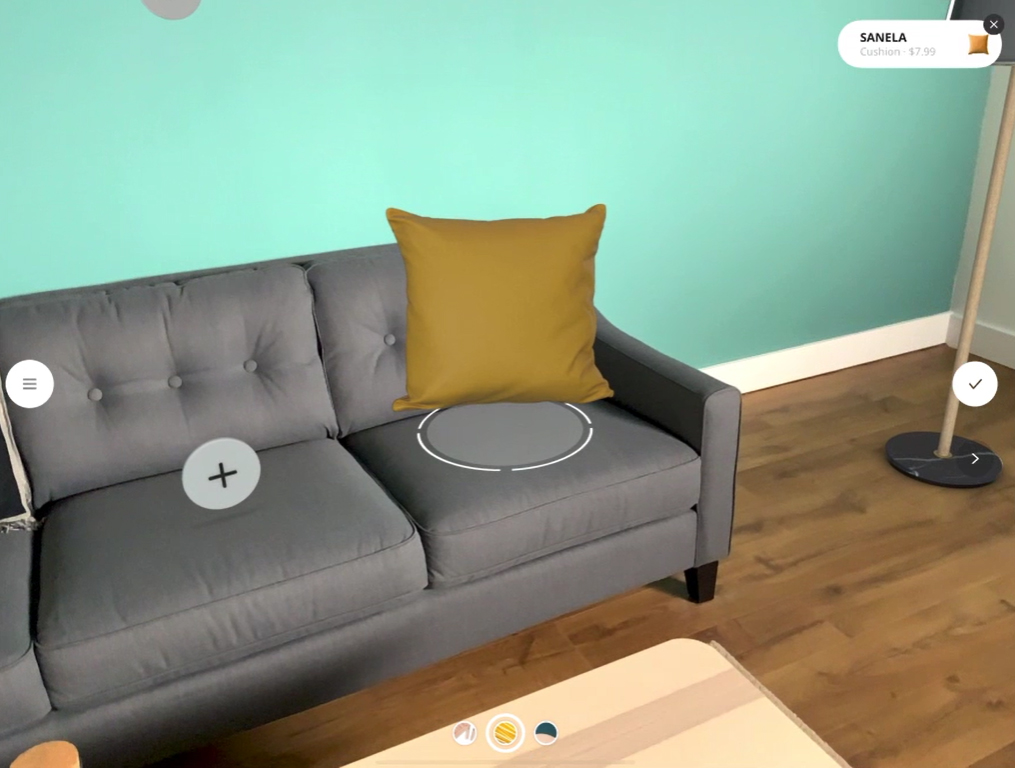
\includegraphics[scale=0.25]{Images/Estado del arte/ikeaAR.jpg}
    \caption[Aplicación de Apple IKEA Place]{Aplicación de Apple IKEA Place\footnotemark.}
    \label{fig:ikeaAR}
\end{figure}
\footnotetext{Fuente: \url{https://www.apple.com/augmented-reality/}}

En la realidad aumentada o AR (del inglés \textit{Augmented Reality}) los elementos creados por ordenador que se colocan en el mundo real no tienen conocimiento de los elementos que existen en el entorno donde se están posicionando. \\

Existen dos tipos de realidad aumentada~\cite{arwithMarkers}, realidad aumentada con marcadores y realidad aumentada sin marcadores. Los marcadores son imágenes en 2D con símbolos o características especiales que son fáciles de captar (figura~\ref{fig:armaerkersexample}), estos marcadores son usados en la realidad aumentada con marcadores para colocar los objetos virtuales. En cambio, la realidad aumentada sin marcadores utiliza distintos sensores para obtener la información que aporta un marcador.

\begin{figure}[H]
    \centering
    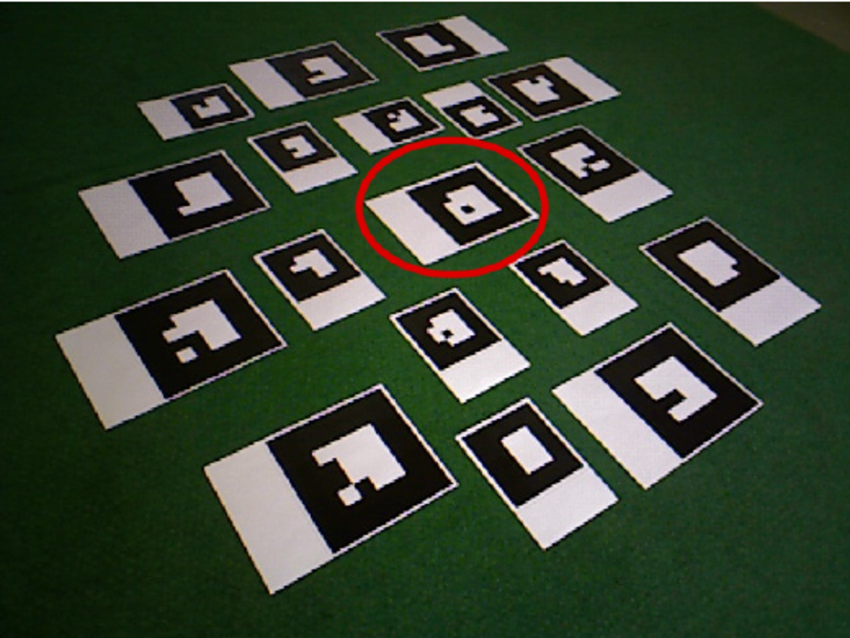
\includegraphics[scale=0.25]{Images/Estado del arte/armarkers.png}
    \caption{Ejemplo de marcadores de AR~\cite{arMarkerArticle}.}
    \label{fig:armaerkersexample}
\end{figure}

Por otro lado, la realidad virtual~\cite{vrintroduction} o VR (del inglés \textit{Virtual Reality}) es una tecnología basada en la simulación de un entorno generado por ordenador que destaca por ser una experiencia inmersiva completa (figura~\ref{fig:superhotVR}). Esto se consigue gracias a la sensación de presencia en el entorno virtual que se genera en el usuario principalmente a través del sentido de la vista y del sonido. En la realidad virtual el usuario se coloca un dispositivo con el que no puede ver nada del mundo físico.

\begin{figure}[H]
    \centering
    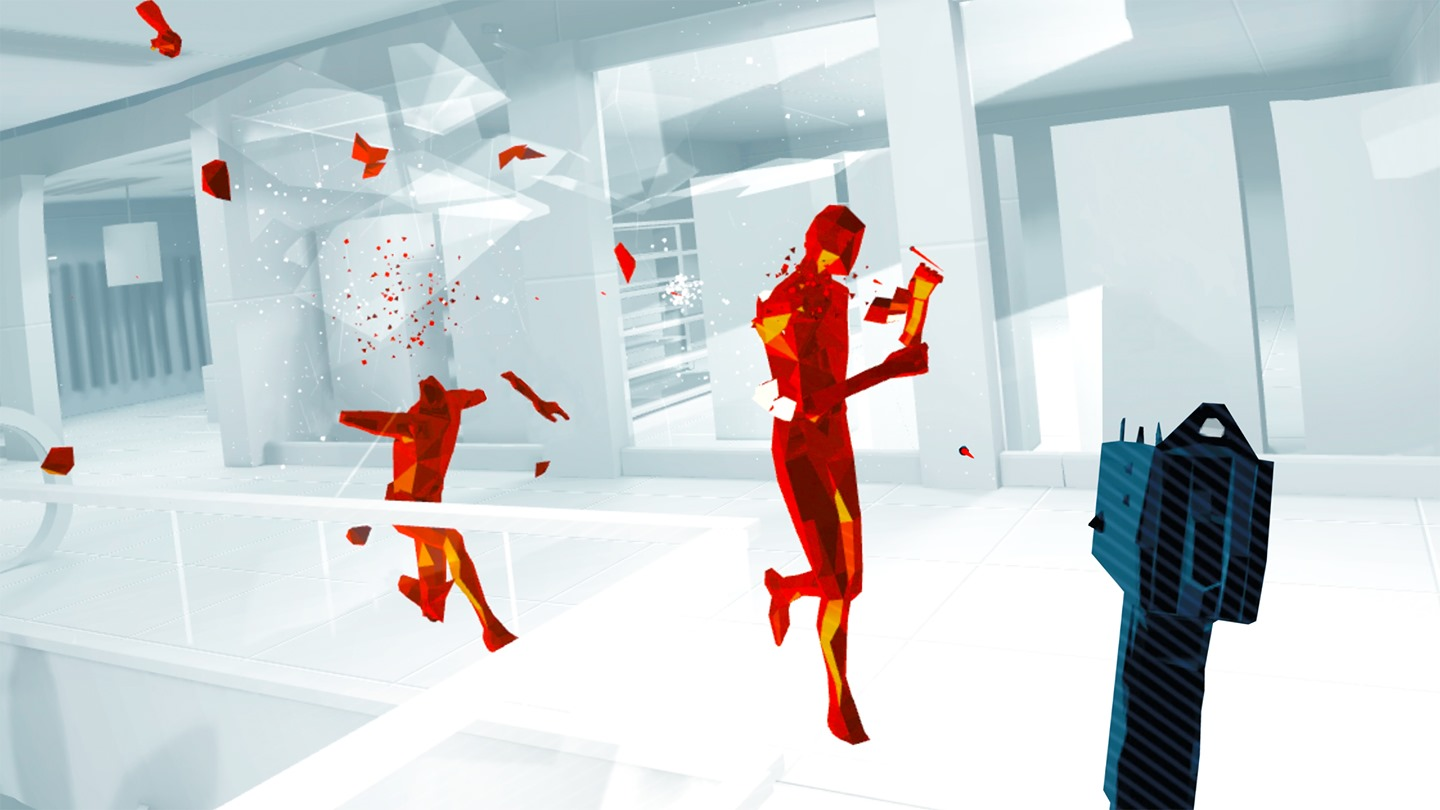
\includegraphics[scale=0.25]{Images/Estado del arte/superhotvr.jpg}
    \caption[Captura del juego de realidad virtual SUPERHOT VR.]{Captura del juego de realidad virtual SUPERHOT VR\footnotemark. El usuario maneja el arma con el que dispara a los enemigos de color rojo.}
    \label{fig:superhotVR}
\end{figure}
\footnotetext{Fuente: \url{https://www.oculus.com/experiences/quest/1921533091289407/}}
A diferencia de la realidad aumentada, en la realidad virtual todos los elementos son conscientes de la existencia de los otros objetos, ya que todo el entorno pertenece a la misma simulación y el mundo real no participa en ella.\\

%superhotVR https://www.oculus.com/experiences/quest/1921533091289407/


Por otra parte, se conoce como realidad mixta o MR (del inglés \textit{Mixed Reality}) a la combinación de realidad virtual y realidad aumentada, es decir, a la fusión de la interacción entre elementos físicos y virtuales (figura~\ref{fig:mrdefinitionexample}). En esta tecnología el usuario está presente en un mundo que es tanto virtual como físico, destacando principalmente la posibilidad de interacción de los objetos virtuales con el entorno físico.\\

\begin{figure}[H]
    \centering
    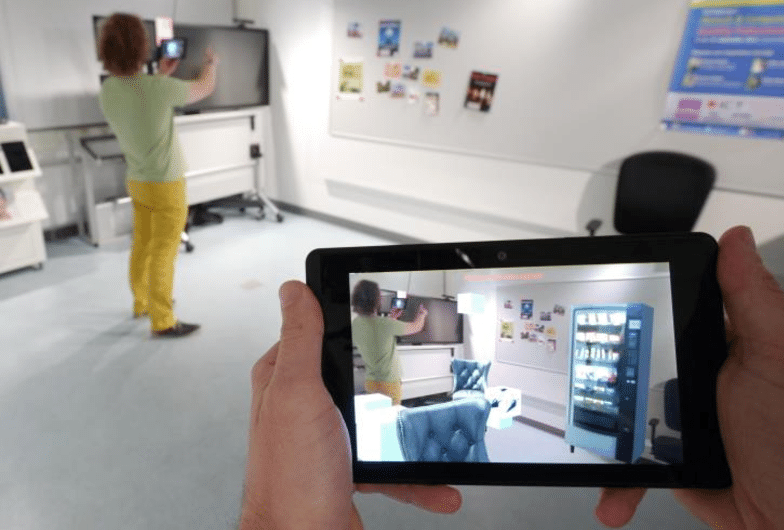
\includegraphics[scale=0.3]{Images/Estado del arte/mrexampledefinition.png}
    \caption{Experiencia colaborativa de MR con dos tabletas~\cite{mrExampleDefinition}. En la tableta se puede ver como se están mostrando elementos virtuales que no existen en el mundo físico mientras la otra persona interactúa con otros elementos de la pared.}
    \label{fig:mrdefinitionexample}
\end{figure}

Fue en 1994 cuando Paul Milgram y Fumio Kishino definieron el concepto del continuo de la virtualización~\cite{ARDisplayofContinuum}. Indican que la realidad mixta se define como el entorno que se encuentra en cualquier punto entre los extremos de éste, es decir, entre la realidad aumentada y la realidad virtual (figura~\ref{fig:rvcontinuumfig}).\\


Por último, se conoce con el término de realidad extendida~\cite{xrintro} o XR (del inglés \textit{eXtended Reality}) a la tecnología que abarca el conjunto de las tres realidades mencionadas anteriormente, realidad aumentada, realidad mixta y realidad virtual.  

\begin{figure}[htbp]
\centering
    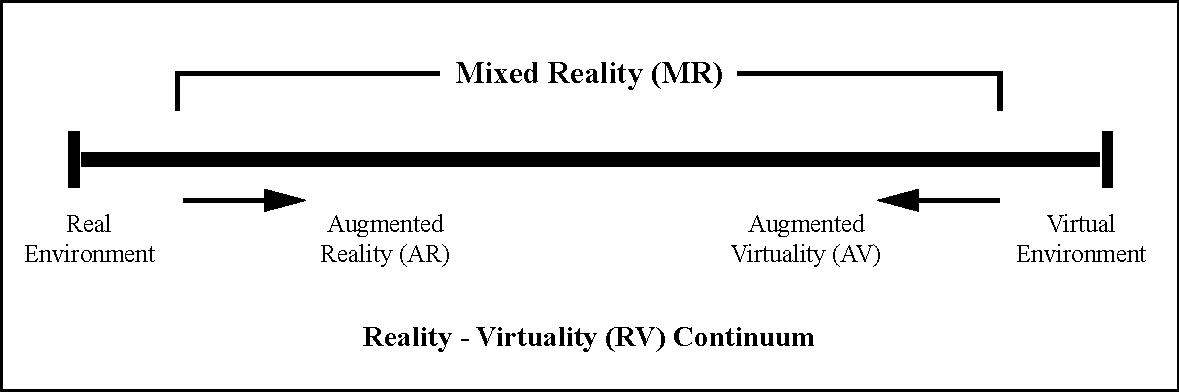
\includegraphics[scale=0.7]{Images/Estado del arte/rvcontinuum.pdf}
    \caption{Reality-Virtualiy Continuum \cite{ARDisplayofContinuum}.}
    \label{fig:rvcontinuumfig}
\end{figure}







\parindent=0em
\section{Necesidades tecnológicas}
\noindent

Las distintas realidades abarcadas en las XR utilizan distintos tipos de tecnologías para poder crear las experiencias respectivas a cada realidad. \\

\parindent=0em
\subsection{Tecnologías en realidad aumentada}
\noindent


En primer lugar, un sistema básico de realidad aumentada~\cite{arhardwarerequirements} está formado al menos por tres tipos de elementos: sensores, procesadores y \textit{displays}. Los sensores son los encargados de obtener información del entorno y transmitírsela a la aplicación, los procesadores gestionan dicha información y los \textit{displays} son los dispositivos en los que se muestra la información de la aplicación.\\

Existen distintos tipos de sensores como los que aportan información sobre el nivel de luz del ambiente o la temperatura, aun así, los sensores más importantes son los que generan información sobre posición y orientación para conocer la pose y ubicación del usuario, este seguimiento del usuario se conoce como \textit{tracking}.\\

Se pueden distinguir distintos tipos de \textit{tracking} en función de los componentes que se utilicen para generar la información referente al usuario. Esta búsqueda de la pose del usuario se puede dividir~\cite{tracking1} en las siguientes técnicas:  

\begin{itemize}
    \item \textbf{Técnicas basadas en sensores:} Se utilizan sensores magnéticos, acústicos, inerciales o mecánicos entre otros. Por ejemplo, el \textit{tracking} con sensores mecánicos se realiza atando enlaces al objeto el cual se quiere realizar este seguimiento. Los enlaces tienen sensores que aportan información sobre el ángulo que se forma entre la unión de varios enlaces.\\
    
    %potenciometro https://www.iberobotics.com/producto/potenciometro-lineal-b10k-10k/
    
    Normalmente se utiliza un potenciómetro (figura \ref{fig:potenciometro}) en las uniones para obtener el voltaje, de este modo, cuando el ángulo entre los enlaces cambia, varía la resistencia del potenciómetro haciendo que cambie el valor del voltaje. Gracias a este componente se puede conocer la posición y orientación del objeto.
    
    \begin{figure}[H]
    \centering
    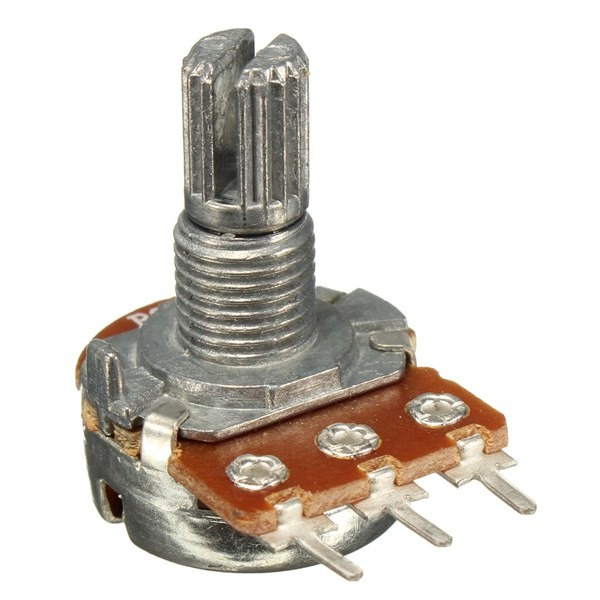
\includegraphics[scale=0.14]{Images/Estado del arte/potenciometro.jpg}
    \caption{Potenciómetro.}
    \label{fig:potenciometro}
\end{figure}

    Por otra parte, el seguimiento mediante sensores magnéticos~\cite{magneticIntro} es otra de las opciones del \textit{tracking} con sensores. El \textit{tracking} magnético se basa en la generación de un campo magnético de un transmisor para medir dicho campo en un receptor colocado en el objeto al cual se quiere hacer el seguimiento~\cite{magneticExplanation}. De esta forma se calcula la posición del objeto en relación al transmisor.\\
    
    Los campos magnéticos generados por el emisor pueden ser distorsionados por cualquier elemento metálico cercano, es por ello que este proceso no es una forma de seguimiento fiable por si sola para calcular la pose del objeto de forma exacta, ya que genera error en su estimación.\\
    

    \item \textbf{Técnicas basadas en la visión:} Estas son las técnicas más comunes, en ellas, se utiliza la visión por computador para obtener la información sobre el usuario. La visión por computador o visión artificial~\cite{visionporcomputador} es la transformación de datos de una cámara a una nueva representación, además, es necesario que estos datos incluyan información sobre la posición de la cámara (si se encuentra encima de un vehículo, por ejemplo).\\
    
    Dicha visión por computador se basa en encontrar una correspondencia entre puntos característicos de la imagen 2D y el entorno en 3D. De esta forma, la pose del elemento del cual se quiere hacer el seguimiento, se puede obtener proyectando las coordenadas 3D de los puntos característicos sobre las coordenadas de la imagen 2D y minimizando la distancia hacia estos.
    
    \item \textbf{Técnicas híbridas:} Las técnicas híbridas surgen de la necesidad de una precisión mayor en algunas aplicaciones debido a la robustez de las mediciones que se obtienen al hacer \textit{tracking} mediante sensores o por visión. Se llegó a la conclusión de que se podían combinar las técnicas por sensores con las técnicas que utilizan visión por computador, de esta manera, se saca partido a la velocidad de los sensores frente a la visión por computador y se complementa la robustez de los sensores con la precisión de las técnicas por visión. 
    
    Estas combinaciones permiten afinar el \textit{tracking}, por ejemplo, en una aplicación en el exterior en entornos como ciudades~\cite{hybridtrackingUrban} donde el nivel de distorsión es elevado y los sensores utilizados tradicionalmente (GPS y brújula magnética) son imprecisos.
    
    Para finalizar, un ejemplo de modelo híbrido es el modelo que combina información obtenida por el giroscopio y visión por computador basada en líneas~\cite{robustHybridmodel}, en él, se hace uso del giroscopio para predecir la orientación y la posición de las líneas de las imágenes que luego corrige la visión por computador.
    
\end{itemize}

Otra técnica comunmente utilizada en realidad aumentada es la tecnología SLAM~\cite{arSLAM} (del inglés Simultaneous Localization and Mapping) la cual consiste en una serie de algoritmos utilizados para calcular la posición del objeto del cual se hace el seguimiento, además, realiza una reconstrucción 3D del entorno. En el caso de estar utilizando un dispositivo móvil a la hora de aplicar SLAM se utiliza la información de la cámara, acelerómetro y giroscopio, también, puede complementarse esa información con la obtenida del GPS, sensores de luz o incluso cámaras de profundidad.
\parindent=0em
\subsection{Tecnologías en realidad virtual}
\noindent

En el caso de la realidad virtual es necesario tener en cuenta otros factores para una buena experiencia aparte de la posición y orientación del usuario, como por ejemplo, la posición y gestos de las manos o la distancia interpupilar.\\

Primero de todo, hay que tener en cuenta el concepto de DoF (del inglés \textit{Degrees of Freedom}), los DoF hacen referencia a los distintos movimientos o rotaciones que puede tener en cuenta o realizar un elemento. En los dispositivos de realidad virtual se distingue entre 3DoF y 6DoF (figura~\ref{fig:3dofvs6dof}), por ejemplo, en un dispositivo con 3DoF, solo se tiene en cuenta la rotación mientras que si posee 6DoF se tiene en cuenta estas 3 rotaciones y el movimiento del dispositivo en 3 ejes.\\

\begin{figure}[H]
    \centering
    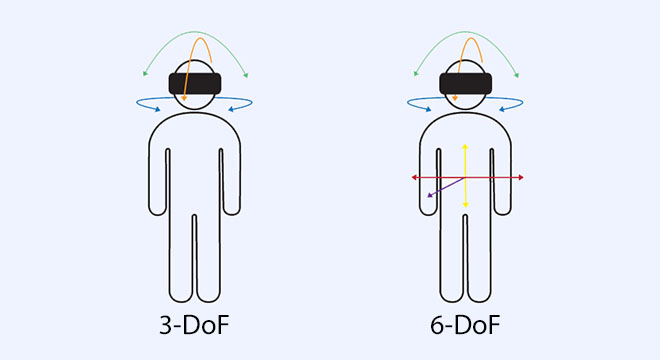
\includegraphics[scale=0.6]{Images/Estado del arte/3dofvs6dof.jpg}
    \caption[Diferenciación entre 3DoF y 6DoF]{Diferenciación entre 3DoF y 6DoF\footnotemark.}
    \label{fig:3dofvs6dof}
\end{figure}
\footnotetext{Fuente: \url{https://virtualspeech.com/blog/degrees-of-freedom-vr}}
%https://virtualspeech.com/blog/degrees-of-freedom-vr

Por otra parte, el \textit{hand tracking} o seguimiento de manos es un proceso mediante el cual se obtiene la posición de las manos y también, los gestos que están realizando como cerrar el puño o agarrar algo, entre otros. Un modelo que se presenta para hacer este seguimiento~\cite{robustHandTracking} habla de la dificultad del proceso debido a la gran cantidad y variación de DoF que pueden tomar las manos. Este modelo se basa en una única cámara de profundidad mediante la cual obtienen imágenes que luego procesan utilizando aprendizaje automático para finalmente poder obtener la posición de las manos y su rotación en tiempo real.\\

Aunque no es obligatorio para un correcto funcionamiento de la realidad virtual que los dispositivos utilicen \textit{hand tracking} (ya que se puede utilizar un par de mandos en su lugar) es un factor que incrementa la inmersión del usuario notablemente, asimismo, no es obligatorio el uso de \textit{eye tracking} o seguimiento de ojos pero puede ser beneficioso para la experiencia. Gracias al \textit{eye tracking} se puede obtener información útil~\cite{eyetrackingVR} como las regiones de interés del espacio 3D y saber en qué momento se ha mirado hacia estas regiones, también, se puede cambiar la información en pantalla basándose en dónde está mirando el usuario o incluso controlar las interfaces virtuales con la mirada.\\

%https://www.vistaoftalmologos.es/realidad-virtual-atencion-los-ojos/#:~:text=En%20los%20juegos%20de%20realidad,confuso%2C%20reconstruye%20una%20imagen%20%C3%BAnica.&text=Para%20continuar%20viendo%20la%20pel%C3%ADcula,la%20convergencia%20y%20la%20acomodaci%C3%B3n.

Cuando se hace uso de un visor de realidad virtual, cada ojo obtiene una imagen ligeramente desplazada en el espacio, lo que provoca que el cerebro reconstruya una imagen única. La distancia interpupilar o IPD (del inglés \textit{Interpupillary Distance}) es otro factor a tener en cuenta a la hora de una experiencia virtual satisfactoria debido al proceso del cerebro de crear dicha imagen única. La IPD es la distancia (normalmente medida en milímetros) entre los centros de los dos ojos (figura~\ref{fig:IPDExample}).

\begin{figure}[H]
    \centering
    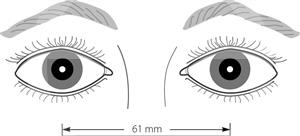
\includegraphics[scale=1]{Images/Estado del arte/IPD.jpg}
    \caption[Medición de la distancia interpupilar]{Medición de la distancia interpupilar\footnotemark.}
    \label{fig:IPDExample}
\end{figure}

\footnotetext{Fuente: \url{https://www.aao.org/image/interpupillary-distance-2}}
Según un estudio realizado con distintas personas haciendo variaciones de la IPD~\cite{IPDTest} en un HMD (del inglés \textit{Head Mounted Display}) o casco de realidad virtual, se llegó a la conclusión de que no había alteraciones a la hora de distinguir los tamaños de los objetos virtuales o afectaciones en la claridad de la visión, en cambio, los usuarios notaron una mayor fatiga con una configuración en el HMD de 50mm y 74mm en la distancia interpupilar en comparación a un valor de la IPD adecuado a su distancia interpupilar anatómica.\\
%https://www.aao.org/image/interpupillary-distance-2

También está relacionado con la visión el concepto de FOV, del inglés \textit{Field Of View}. El FOV hace referencia a la amplitud del campo de visión que ofrece el dispositivo, los seres humanos pueden llegar hasta 180\degree~ gracias a los dos ojos.\\

Para finalizar, respecto a la autonomía de los dispositivos, estos pueden ser inalámbricos o depender de algún cable como fuente de energía. Los dispositivos inalámbricos suelen utilizar pilas o baterías recargables con distintos tiempos de autonomía y en caso de necesitar conectarse a un dispositivo utilizan \textit{bluetooth}. En el caso de no ser inalámbricos los dispositivos suelen conectarse a un ordenador a través de cables HDMI y USB y utilizarlo como fuente de energía.











\parindent=0em
\section{Dispositivos}
\noindent

%https://editeca.com/realidad-mixta/
Dado que la realidad aumentada y la realidad virtual tienen distintas necesidades tecnológicas como se ha tratado en la sección~\ref{sec:necesidadesTecnologicas}, sus dispositivos correspondientes también tienen componentes hardware distintos para satisfacer estas necesidades tecnológicas.\\

En el sector de la realidad aumentada destaca principalmente el uso de teléfonos móviles gracias a su fácil disponibilidad y a la facilidad añadida de crear aplicaciones para estos gracias a la aparición de las tecnologías ARCore y ARKit, además, se puede disfrutar de esta experiencia usando gafas de realidad aumentada y HMDs.\\

Por otra parte, en el campo de la realidad virtual destacan los HMD. Estos dispositivos son variados entre ellos en cuanto a los sensores, cámaras o conectividad entre otras características.\\

Al ser la realidad mixta una combinación entre las dos realidades mencionadas anteriormente, la MR puede ser utilizada a través de cascos enfocados a experiencias de realidad virtual (aunque estos cascos no se van a tratar en esta sección), dispositivos enfocados para su uso en realidad aumentada o incluso desde teléfonos móviles.\\

Del mismo modo, se pueden distinguir dos tipos de dispositivos específicos de realidad mixta en el campo de los HMD. Por un lado los cascos en los que se ve directamente el mundo físico y por otro aquellos HMD en los que la visión del usuario está completamente tapada por el casco y se ve el mundo real a través de las cámaras del dispositivo.\\

%https://www.microsoft.com/en-us/mixed-reality/windows-mixed-reality?rtc=1


También, cabe destacar que un gran número de dispositivos de realidad mixta se utilizan a través de la plataforma WMR\footnotemark~  (\textit{Windows Mixed Reality}). Esta plataforma ofrece acceso a numerosas aplicaciones de realidad mixta y realidad virtual. Para poder hacer uso de WMR es necesario un ordenador con Windows~10 y una tarjeta gráfica y procesador potentes.\\

\footnotetext{\url{https://www.microsoft.com/en-us/mixed-reality/windows-mixed-reality}}


Por último, los teléfonos móviles están empezando a ganar importancia en el sector de la realidad mixta. Según un estudio realizado por Sam Barker \cite{juniperArMrmoney}, los avances en el \textit{Edge Computing}~\cite{edgeComputing}, un paradigma que permite que los servicios de computación en la nube~\cite{cloudComputing} (tecnología de computación que provee unidades computacionales de bajo coste) sean más cercanos al usuario final, y la aparición de las redes de 5G (la quinta generación de tecnología inalámbrica la cual se caracteriza por un aumento de la velocidad y menor latencia frente al 4G), acelerarán el desarrollo de la tecnología de realidad mixta en móviles.\\

Dicho autor afirma que las conexiones inalámbricas que se utilizan hoy día para procesar la información de los dispositivos, deberán alcanzar velocidades mayores (usando el 5G) para una experiencia inmersiva total, además, calcula que gracias a estos avances se alcanzará un mercado de~43 billones de dólares en el año~2024, a diferencia de los 8 billones alcanzados en~2019.

\parindent=0em
\subsection{Teléfonos móviles}
\label{sec:telefonosMoviles}
\noindent

%https://www.aniwaa.com/product/vr-ar/tesseract-holoboard-enterprise-edition/

Los teléfonos móviles son un gran dispositivo ya que combinan GPS, cámara, brújula y un acelerómetro, cubriendo así las necesidades de una aplicación de realidad aumentada~\cite{arsmartphones}. El teléfono móvil es un dispositivo muy común entre la población lo cual facilita el desarrollo y expansión de esta realidad. Por otro lado, dichos dispositivos se pueden utilizar también para realidad mixta utilizando unos cascos en los que se introduce el móvil para generar una experiencia de MR.\\

Existen distintos HMD que se utilizan para estas experiencias de realidad mixta acoplando los móviles a alguna parte de las gafas, como por ejemplo, las \textit{Holoboard Enterprise Edition} de la mano de la empresa \textit{TESSERACT} (figura~\ref{fig:mrandroidTESSERACT}). Este dispositivo es compatible a partir de Android 6.0  y como especificaciones técnicas se pueden destacar sus 82\degree~ de FOV, utiliza la tecnología SLAM para el \textit{tracking}, posee un controlador 6DoF y utiliza el \textit{tracking} por sensores IMU, además, permite experiencias colaborativas en la nube.

\begin{figure}[H]
    \centering
    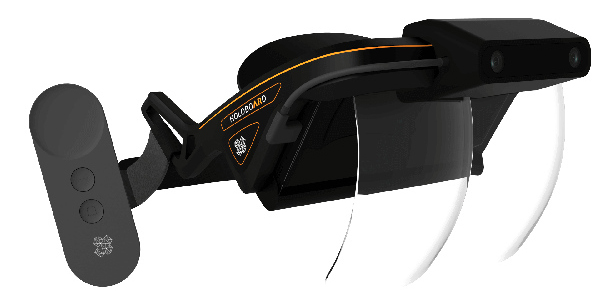
\includegraphics[scale=0.3]{Images/Estado del arte/mrandroid.jpg}
    \caption[\textit{Holoboard Enterprise Edition}]{
    \textit{Holoboard Enterprise Edition\footnotemark.}
    }
    \label{fig:mrandroidTESSERACT}
\end{figure}
\footnotetext{Fuente: \url{https://www.aniwaa.com/product/vr-ar/tesseract-holoboard-enterprise-edition}}
En cambio, si estamos hablando de un dispositivo para utilizar en móviles con iOS podemos hablar del casco \textit{Bridge} (figura~\ref{fig:mriosBRIDGE}) de la empresa \textit{Occipital}. Este HMD requiere de un componente extra llamado \textit{Occipital Structure Sensor}, el cual, se utiliza para el escaneo 3D del entorno.

\begin{figure}[H]
    \centering
    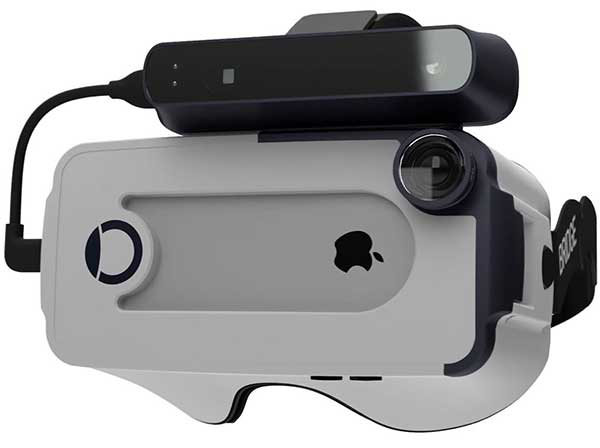
\includegraphics[scale=0.3]{Images/Estado del arte/mrios.jpg}
    \caption[\textit{Occipital Bridge}]{\textit{Occipital Bridge\footnotemark.}}
    \label{fig:mriosBRIDGE}
\end{figure}

\footnotetext{Fuente: \url{https://www.aniwaa.com/product/vr-headsets/occipital-bridge/}}

Las gafas \textit{Bridge} tienen un FOV de 120º, un controlador de 6DoF y destacan por que gracias a estas se puede utilizar aplicaciones de realidad aumentada, realidad mixta y realidad virtual, también, utiliza la técnica de \textit{tracking} conocida como \textit{inside-out}.\\

Pese a que la principal diferencia entre las dos gafas es el sistema operativo para el que están destinadas, se puede observar que los precios son similares y que las gafas destinadas para iOS poseen un FOV notablemente superior.


\begin{table}[H]
\centering
\renewcommand{\arraystretch}{1.5}
\begin{tabular}{llllll}
\toprule
Dispositivo                  & Precio & DoF & FOV & \textit{SO} & \textit{Tracking} \\
\midrule
\textit{Holoboard Enterprise Edition} & \$399  & 6DoF         & 82\degree           & Android     & SLAM              \\
\textit{Occipital Bridge }            & \$349  & 6DoF         & 120\degree          & iOS         & \textit{Inside-out}\\\bottomrule       
\end{tabular}
\caption{Comparación entre ambas gafas de \textit{MR} para móviles.}
\label{cuadro:comparacionphonesMR}
\end{table}


\parindent=0em
\subsection{Hololens 2}
\label{HoloLens2Dispositivo}
\noindent

Las \textit{HoloLens 2} (figura~\ref{fig:vistasHoloLens2}) son un casco desarrollado por \textit{Microsoft} que salió al mercado en 2019. Es un dispositivo dotado de tecnología de \textit{eye tracking} y \textit{hand tracking} capaz de detectar las dos manos, esto añade un extra de inmersión a la experiencia y de comodidad ya que no se necesitan mandos para manejarlo y se pueden tener las manos libres. Respecto a los sensores, goza de acelerómetro, giroscopio y magnetómetro para medir la velocidad, orientación y fuerzas gravitacionales del dispositivo.\\


\begin{figure}[htbp]
\centering
    \hspace{-4mm}
    \begin{minipage}{0.5\textwidth}
        \centering
        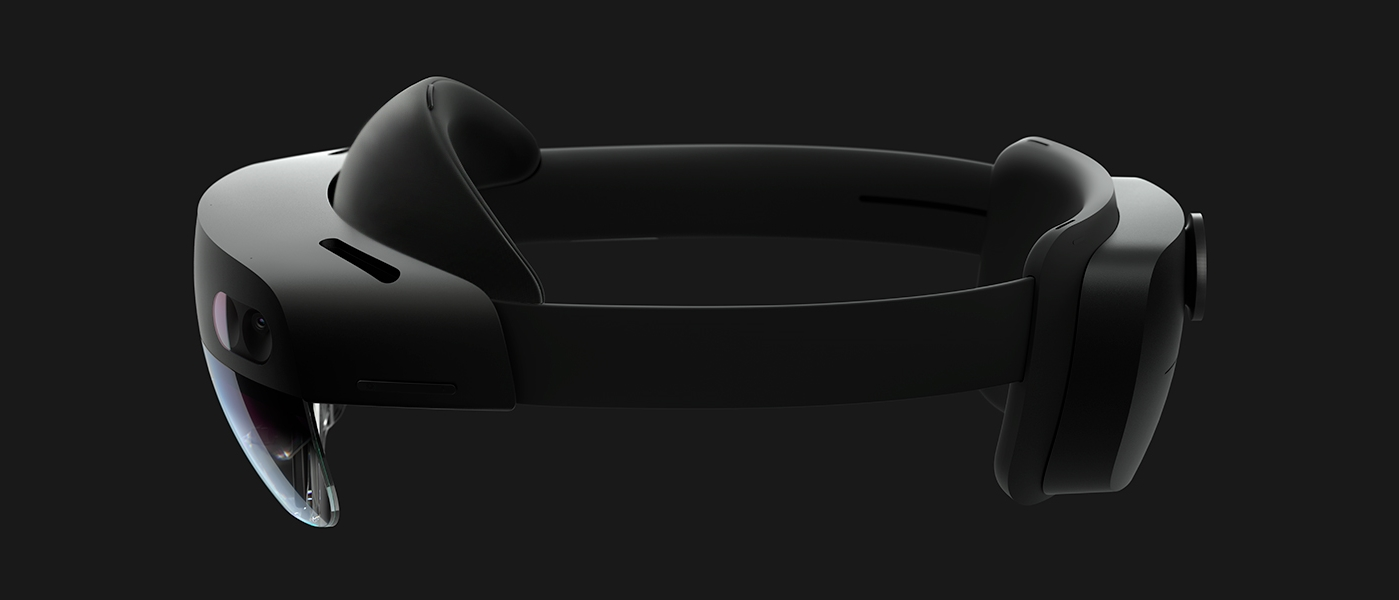
\includegraphics[scale=0.2]{Images/Estado del arte/hololens2_2.jpeg}\\
        (a) Vista lateral.
    \end{minipage}
    \begin{minipage}{0.5\textwidth}
        \centering
        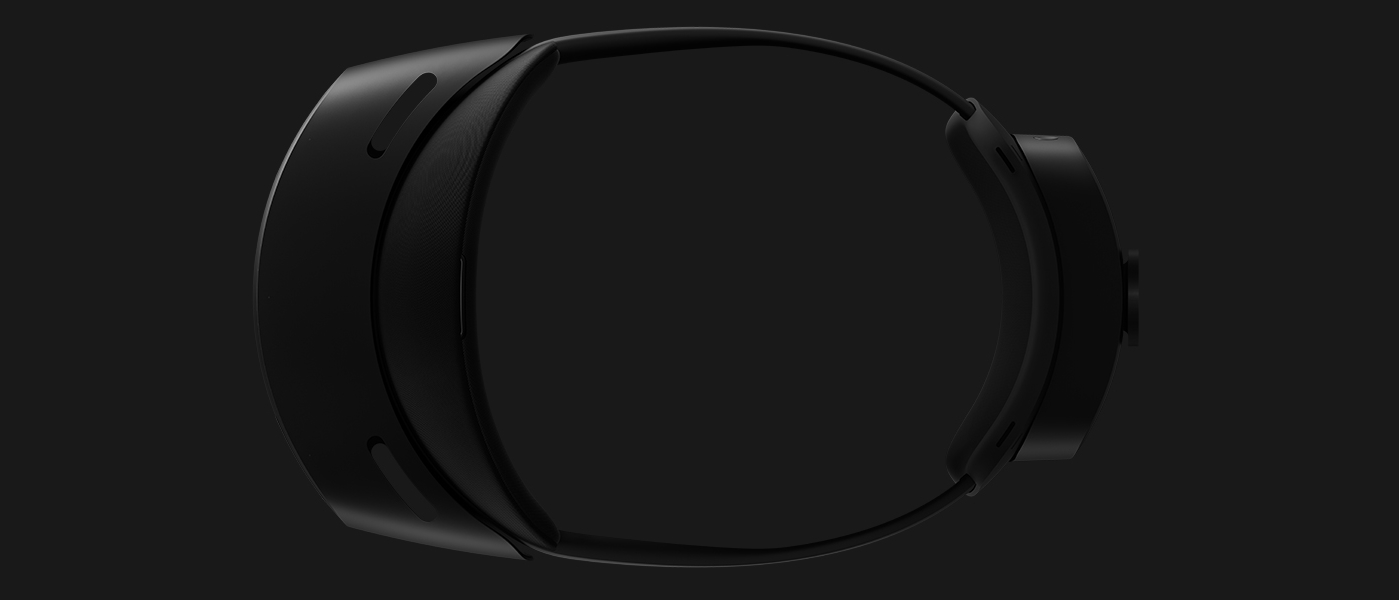
\includegraphics[scale=0.2]{Images/Estado del arte/hololens2_3.jpeg}\\
       (b) Vista superior.
    \end{minipage}\\
    \caption{Vistas de las Microsoft HoloLens 2\textsuperscript{\ref{hololens2footer}}.}
    \label{fig:vistasHoloLens2}
\end{figure}


Las \textit{Hololens 2} funcionan de forma independiente ya que tienen integrado su propio procesador y utilizan una batería recargable con una autonomía de entre 2 y 3 horas, además, permiten capturar el movimiento y los giros del usuario gracias a su control de \textit{6DoF}. Por otra parte, respecto a la conectividad, este \textit{HMD} tiene \textit{WiFi}, \textit{bluetooth} y permite conexiones mediante un \textit{USB} tipo C. Por ejemplo, se puede utilizar la conexión \textit{WiFi} para navegar por internet (a través del navegador \textit{Microsoft Edge} incorporado en las gafas) o para conectarse a reuniones en línea con otros usuarios de las mismas gafas.\\

Del mismo modo, este casco  está diseñado con un sistema ergonómico de tal forma que no hay necesidad de quitarse las gafas, ya que se puede colocar directamente sobre ellas (figura~\ref{fig:hololensErgonomicas}).\\


\begin{figure}[H]
    \centering
    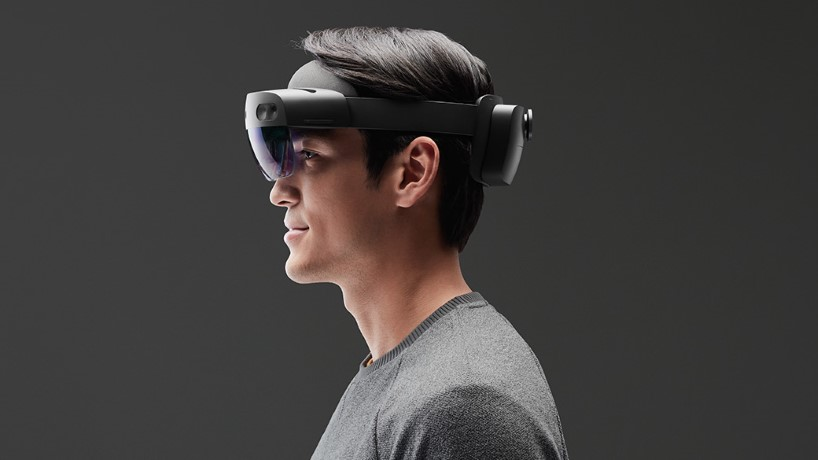
\includegraphics[scale=0.35]{Images/Estado del arte/hololens2_1.jpeg}
     \caption{Diseño ergonómico del dispositivo\textsuperscript{\ref{hololens2footer}}.
  }
  \label{fig:hololensErgonomicas}
\end{figure}


Para finalizar, este \textit{HMD} tiene un \textit{FOV} de 43º, una resolución de 2.048×1.080 píxeles por ojo (4.096x1.080 en combinación) y una \textit{IPD} que se ajusta automáticamente según la posición de los ojos que es detectada por un sensor \textit{IPD}, asimismo, tiene un sensor de~1~Megapíxel de profundidad \textit{ToF} (del inglés Time of Flight, calcula distancias entre objetos en función a la distancia que tarda la emisión y recepción de un haz de luz infrarrojo) y un peso de 566 gramos.  


%https://www.microsoft.com/es-es/hololens/hardware



\parindent=0em
\subsection{HMD Odyssey+}
\label{sec:odyssey}
\noindent

%https://www.samsung.com/hk_en/news/product/reality-headset-hmd-odyssey-plus/

El casco \textit{HDM Odyssey+} (figura~\ref{fig:hdmOdysseyVista}) es un dispositivo desarrollado por la empresa \textit{Samsung} que salió al mercado en 2018, no es un casco independiente ya que requiere estar conectado a un ordenador compatible con la plataforma \textit{Windows Mixed Reality} para funcionar, se conecta al ordenador mediante un cable \textit{HDMI}~2.0 y un \textit{USB}~3.0.

\begin{figure}[h]
    \centering
    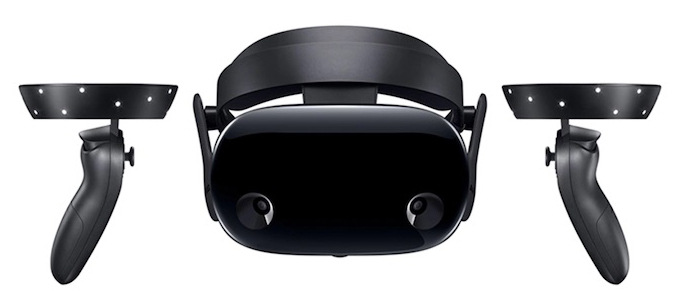
\includegraphics[scale=0.6]{Images/Estado del arte/samsungOdysseyplus.jpg}
    \caption{HDM Odyssey+ dispositivo al completo.}
    \label{fig:hdmOdysseyVista}
\end{figure}

En cuanto a la parte de monitorización de la imagen, este casco tiene una resolución de 1.440 x 1.600 píxeles por ojo, un total de 2.880 x 1.600 píxeles combinando los dos ojos, además, el \textit{Field of View} abarca un total de 110º. Este dispositivo no posee tecnología de \textit{hand tracking} (por lo que controla el movimiento de manos con dos mandos que funcionan con pilas) y tampoco tiene \textit{eye tracking}, en cambio, destaca por tener dos sensores \textit{6DoF} frente al único que tiene, por ejemplo, las \textit{Hololens~2} (sección~\ref{HoloLens2Dispositivo}).\\

Por otra parte, está dotado de sensores como acelerómetro, giroscopio, brújula y sensor de proximidad (este último se utiliza para saber en qué momento se lleva puesto el casco), del mismo modo, posee una diadema que se puede  modificar para ajustar el casco a la cabeza de cada individuo, sin embargo, este dispositivo no está diseñado para ser utilizado con gafas.\\ 

Por último, tiene un sensor que ajusta automáticamente la \textit{IPD}, conexión \textit{bluetooth} y un peso total de 644g teniendo en cuenta solo el \textit{HMD} y un añadido de 176g si se cuenta el peso del cable.


\footnotetext[1]{
\label{hdmOdysseyfooter}{Imagen de la HDMOdyssey+: \url{https://www.samsung.com/us/computing/hmd/windows-mixed-reality/hmd-odyssey-windows-mixed-reality-headset-xe800zba-hc1us/}.}}

\footnotetext[1]{
\label{hdmOdysseyfooter}{Especificaciones de la HDMOdyssey+: \url{https://www.microsoft.com/en-us/p/samsung-hmd-odyssey/8n2d0nk20p8m?cid=msft_web_collection&activetab=pivot:techspecstab}.}}
\parindent=0em
\subsection{Magic Leap One}
\noindent

El dispositivo \textit{Magic Leap One}\textsuperscript{\ref{magicLeaponeFotterSpecs}} fue lanzado al mercado el 8 de Agosto de 2018 de manos de la compañía Magic Leap a un precio inicial de 2,295 dólares exclusivamente en Chicago, Los Ángeles, Miami, Nueva York, San Francisco y Seattle .\\

En el ámbito técnico este casco destaca por su ligero peso de 316 gramos frente a los 566 gramos de la HoloLens 2 (sección \ref{HoloLens2Dispositivo}), posee un sistema 6DoF para el tracking, conectividad vía Bluetooth 4.2, WiFi o USB tipo C.\\

\begin{figure}[htbp]
\centering
    \hspace{-4mm}
    \begin{minipage}{0.5\textwidth}
        \centering
        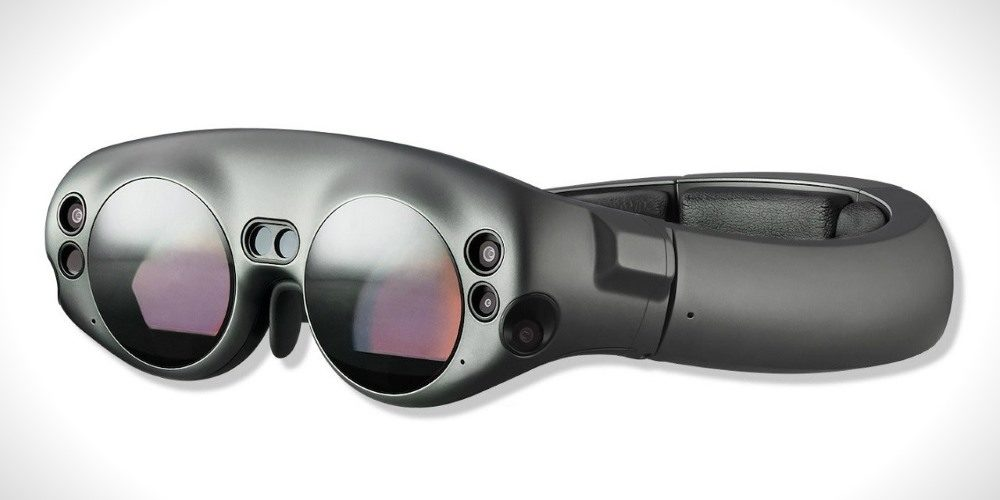
\includegraphics[scale=0.8]{Images/Estado del arte/magicleapone1.jpg}\\
        (a) Vista del casco completo
    \end{minipage}
    \begin{minipage}{0.5\textwidth}
        \centering
        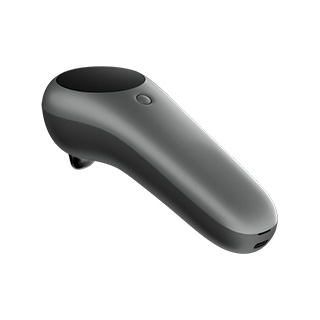
\includegraphics[scale=0.3]{Images/Estado del arte/magicleapone2.jpg}\\
       (b) Vista del mando
    \end{minipage}\\
    \caption{Dispositivo completo de las Magic Leap One\textsuperscript{\ref{magicLeaponeFotterImages}}.}
    \label{fig:vistasMagicLeapnOne}
\end{figure}

Por otro lado, utiliza una CPU (Unidad Central de Procesamiento) dos núcleos Denver 2.0 64-bit y cuatro núcleos ARM Cortex A57 64-bit, una Nvidia Pascal de 256 núcleos CUDA para la GPU (Unidad de Procesamiento Gráfico), tiene 128 Gigabytes como capacidad de almacenamiento y, por último, una batería de litio recargable que permite un uso continuado de 3 horas. 


%https://www.businessinsider.com/magic-leap-one-creator-edition-price-specifications-battery-life-release-date-2018-8?IR=T


\footnotetext[1]{
\label{magicLeaponeFotterSpecs}{Especificaciones obtenidas de \url{https://www.businessinsider.com/magic-leap-one-creator-edition-price-specifications-battery-life-release-date-2018-8?IR=T}.}}

\footnotetext[1]{
\label{magicLeaponeFotterImages}{Imágenes sacadas de \url{https://www.estiloextra.net/magic-leap-one-las-nuevas-y-prometedoras-gafas-de-realidad-aumentada/}.}}

\parindent=0em
\subsection{DAQRI Smart Helmet}
\label{subsec:DAQRISMART}
\noindent

%https://www.linkedin.com/pulse/daqri-smart-helmet-closer-look-nathan-gaydhani

El \textit{DAQRI Smart Helmet} (figura~\ref{fig:vistaDAQRIHelmet}) es un HMD enfocado al uso industrial, está formado por un dispositivo de realidad mixta sin cables integrado en un casco duro (cascos utilizados por ejemplo en la construcción). Ya que está pensado para un uso industrial está dotado de 4 cámaras para poder capturar todo el entorno, es decir, abarcar 360\degree .\\

\begin{figure}[H]
    \centering
    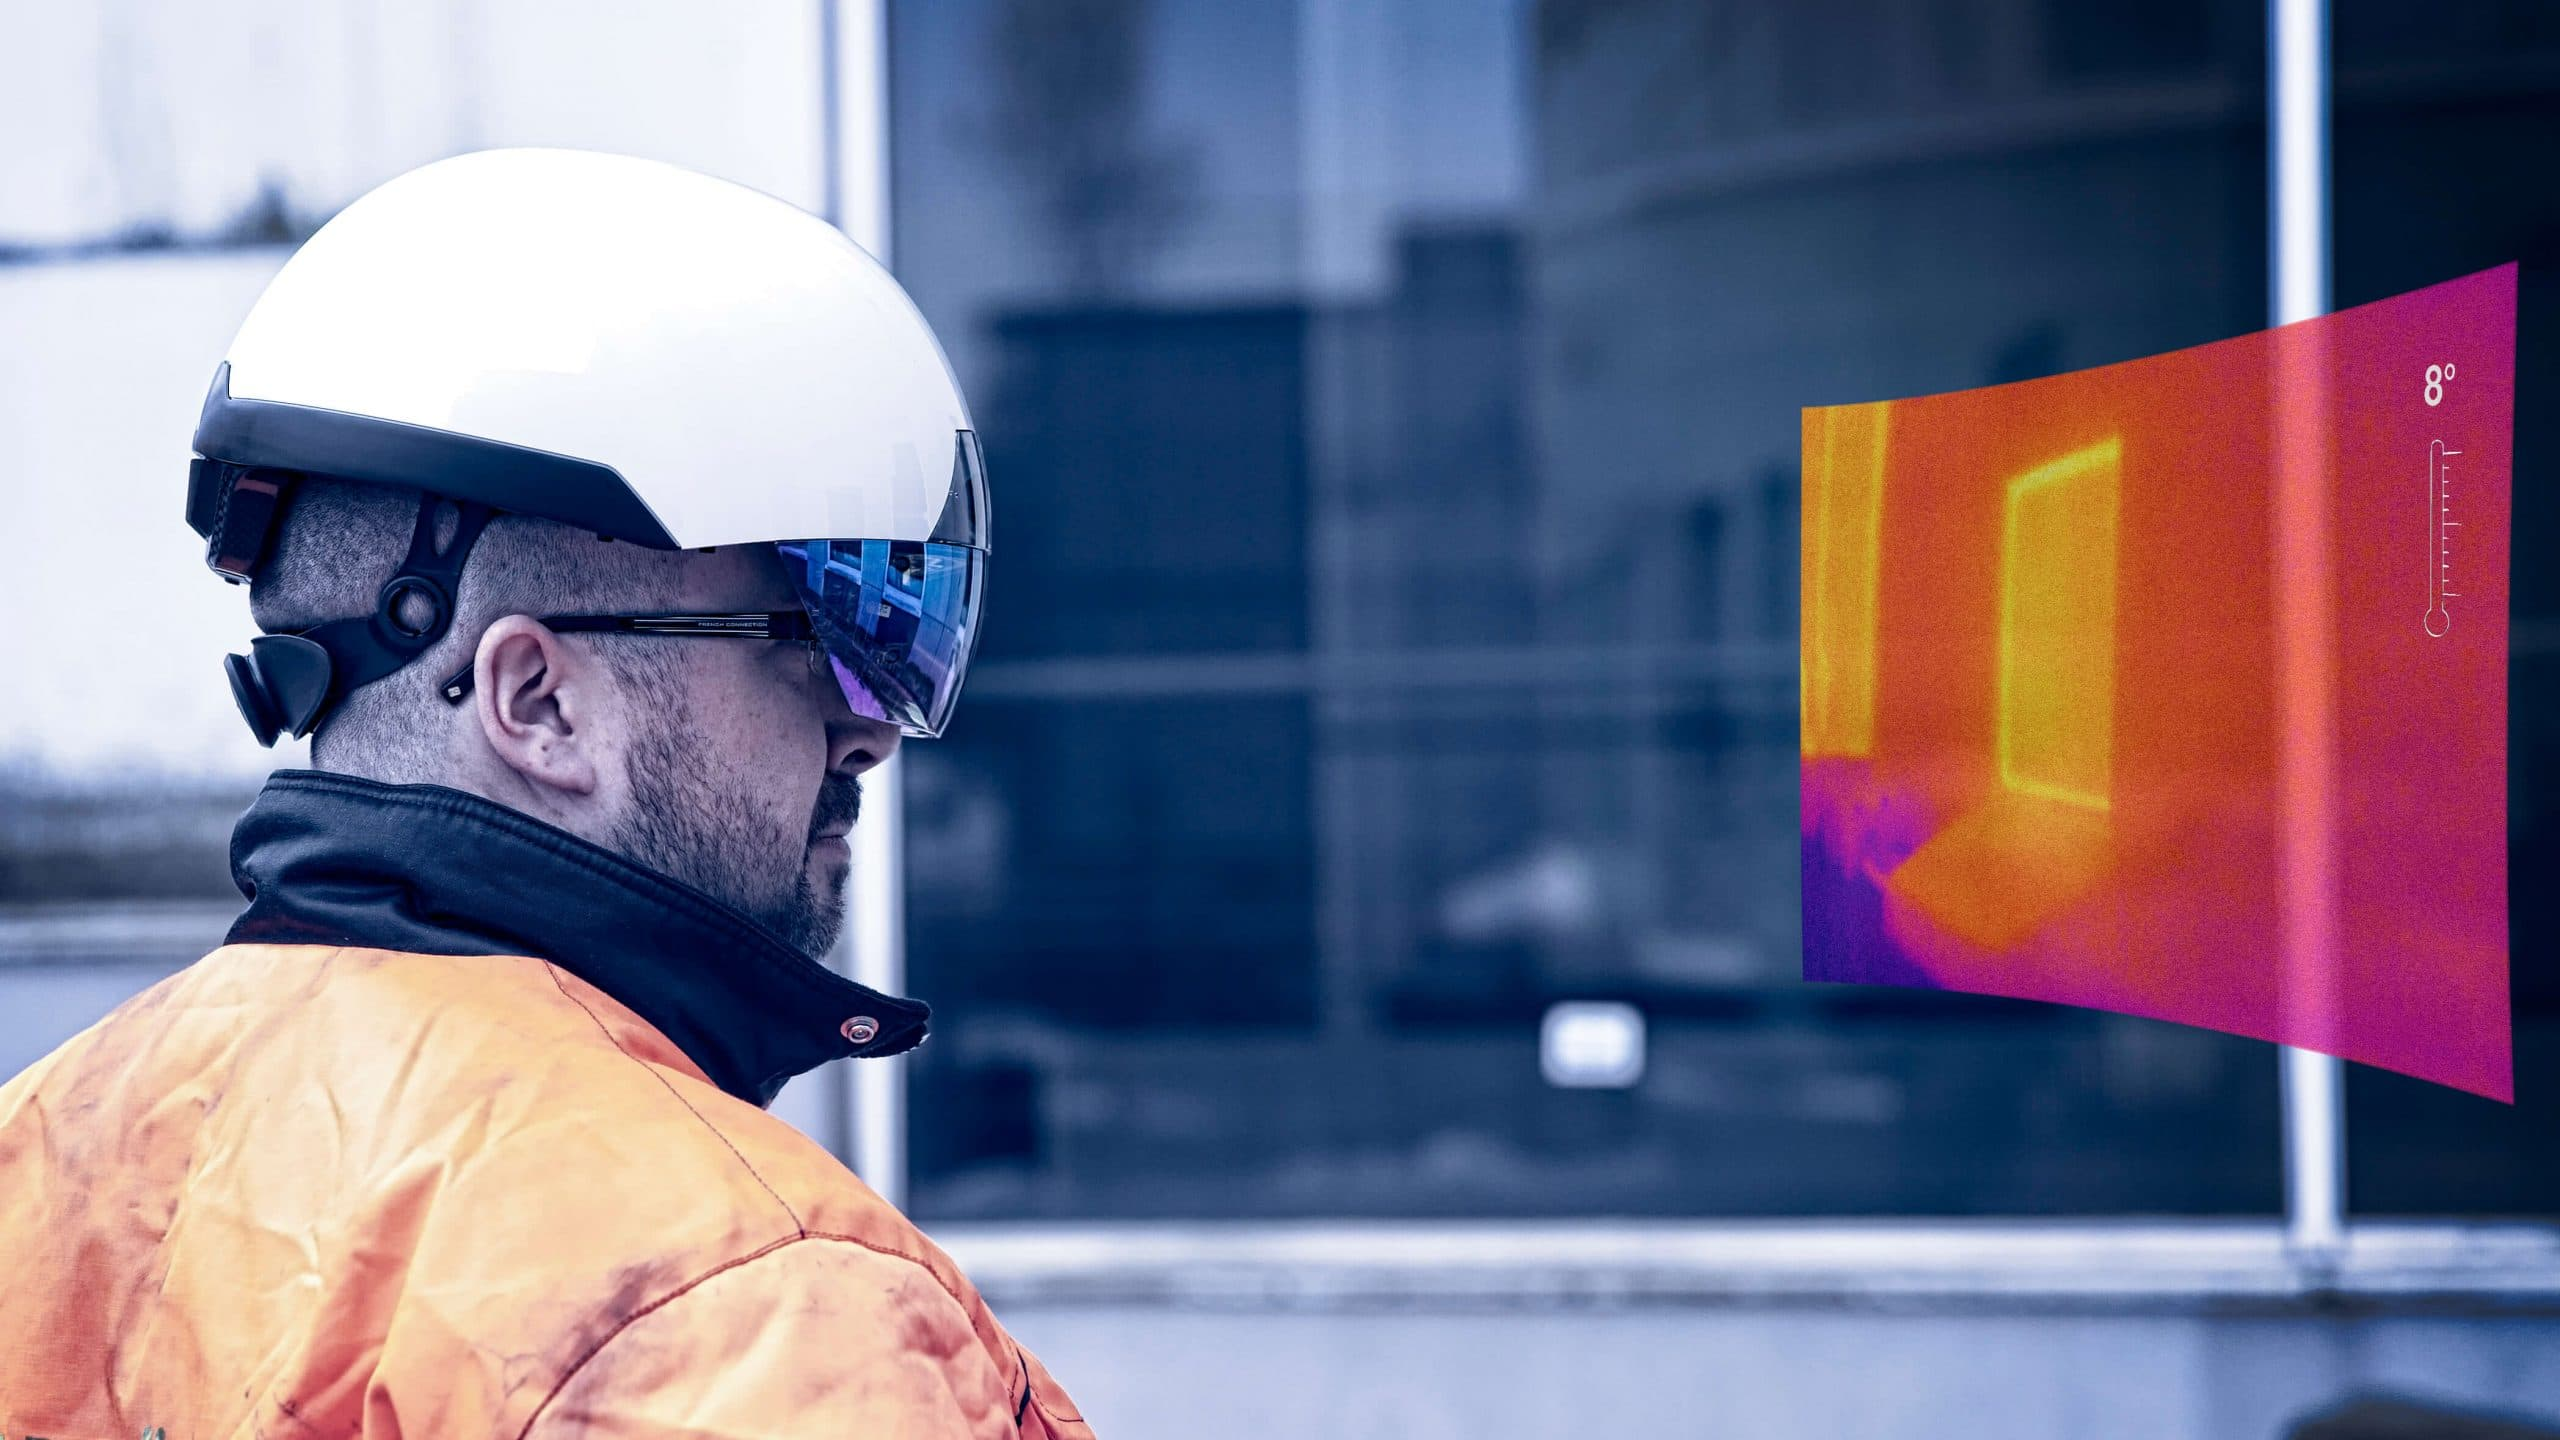
\includegraphics[scale=0.12]{Images/Estado del arte/daqrihelmet.jpg}
    \caption[Vista del \textit{DAQRI Smart Helmet}]{Vista del \textit{DAQRI Smart Helmet}\footnotemark.}
    \label{fig:vistaDAQRIHelmet}
\end{figure}

\footnotetext{Fuente: \href{https://www.stereoscape.com/blog/2017/04/25/daqri-smart-helmet-so-much-more-than-a-helmet/}{\nolinkurl{https://www.stereoscape.com/blog/2017/04/25/daqri-smart-helmet}}}


Con el objetivo de proteger al usuario en entornos industriales peligrosos, el dispositivo cuenta con una cámara termográfica (para poder controlar lugares potencialmente peligrosos debido a su temperatura) y barómetro para poder medir la presión del entorno.\\

Para el seguimiento, el \textit{DAQRI Smart Helmet} utiliza la tecnología SLAM y posee 6DoF para el movimiento y los giros del usuario. Del mismo modo, ya que el objetivo final es proteger al usuario, el dispositivo cuenta con reconocimiento de órdenes por voz y de control de movimientos de la cabeza para manejar el HMD, de esta forma se pueden tener las manos libres.\\


Finalmente, cabe recalcar que el casco goza de procesadores y un sistema operativo Android para ser totalmente independiente, también, utiliza unas baterías intercambiables de 5.700 miliamperios por hora y dispone de conectividad WiFi para poder comunicarse por vídeo en tiempo real remotamente con otros usuarios. El casco tiene un peso total de 1 kilo y~500 gramos y su precio actual es de~15.000 dólares.

%\footnotetext{\label{daqriImagefooter}{Imagenes obtenida de: %\url{https://www.stereoscape.com/blog/2017/04/25/daqri-smart-helmet-so-m%uch-more-than-a-helmet/}.}}




\parindent=0em
\subsection{HP VR1000-127il}
\noindent

Este \textit{HMD} de la empresa \textit{HP} salió al mercado en el año 2018, es un dispositivo dependiente de un ordenador compatible con la plataforma \textit{Windows Mixed Reality}. Este casco se conecta a dicho ordenador a través de una conexión 2 en 1 que combina un \textit{HDMI} 2.0 y \textit{USB} 3.0. \\

Las gafas \textit{HP VR1000-123il} (figura~\ref{fig:hpvr1000}) utilizan dos controladores inalámbricos (que se conectan mediante \textit{bluetooth}) para controlar el movimiento de las manos, estos controladores utilizan 2 pilas AA cada uno. El dispositivo tiene un campo de visión de 90º y una resolución de 1.440×1.440 píxeles por ojo (un total de 2.880x1.440 píxeles con ambos ojos), por otro lado, el casco cuenta con \textit{6DoF} y la \textit{IPD} no se puede regular. 

\begin{figure}[H]
    \centering
    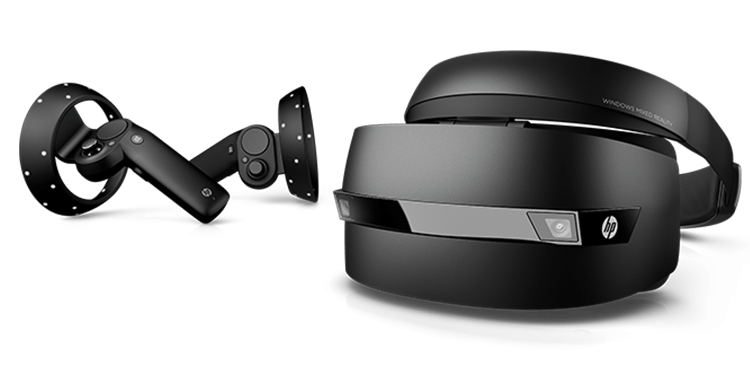
\includegraphics[scale=0.45]{Images/Estado del arte/HP VR1000.png}
    \caption{HP VR1000-123il y sus controladores.}
    \label{fig:hpvr1000}
\end{figure}

Finalmente, este \textit{HMD} no tiene un diseño centrado en su uso con gafas y tiene un peso de 834 gramos. 
\parindent=0em
\subsection{Asus HC102}
\noindent

Este dispositivo (figura~\ref{fig:asushc102}) apareció en el año 2018 de manos de la empresa Asus, al igual que las \textit{HMD Odyssey+} (punto~\ref{sec:odyssey}), es un dispositivo que requiere ser utilizado junto a un ordenador compatible con \textit{Windows Mixed Reality}, está dotado de sensores para calcular la orientación del usuario como giroscopio, acelerómetro, magnetómetro y sensor de proximidad.\\

\begin{figure}[H]
    \centering
    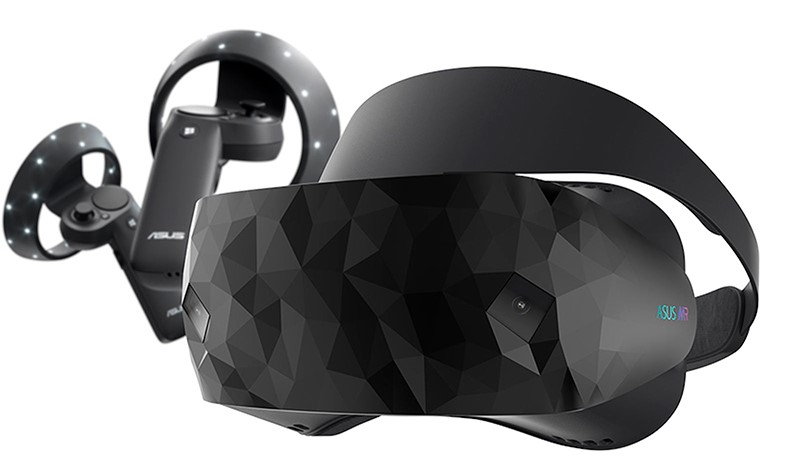
\includegraphics[scale=0.3]{Images/Estado del arte/AsusHC102.jpg}
    \caption[\textit{Asus HC102} al completo]{\textit{Asus HC102} al completo\footnotemark.}
    \label{fig:asushc102}
\end{figure}

\footnotetext{Fuente: \href{https://www.asus.com/Headset/ASUS-Windows-Mixed-Reality-Headset-HC102/specifications/}{\nolinkurl{https://www.asus.com/Headset/ASUSHC102/specifications/}}}

Este casco goza de un FOV de 105\degree , una resolución de 1.440x1.440 por ojo (2.880x1440 en total) y cuenta con dos mandos (cada uno de ellos con un sensor 6DoF) que funcionan con 2 pilas del tipo AA, es decir, 4 pilas AA en total.\\

Finalmente, este HMD permite regular la IPD entre 55mm y 71mm, tiene dos cámaras para hacer un \textit{tracking} de tipo \textit{inside-out} y un peso de 399 gramos.
\parindent=0em
\subsection{Acer AH101-D8EY}
\noindent

Este dispositivo de la marca \textit{Asus} fue lanzado al mercado en el 2017, para utilizarlo es necesario un ordenador compatible con \textit{Windows Mixed Reality}, en cambio, este \textit{HMD} se conecta al ordenador a través de conexión \textit{bluetooth} a diferencia de los otros cascos vistos que se conectan con un cable.\\

El campo de visión del casco es de 100º y respecto a la resolución, es capaz de mostrar 2.880x1.440 píxeles combinando los dos ojos (1.440x1.440 píxeles en cada ojo), además, la distancia interpupilar no es ajustable y viene configurada por defecto a 62mm.\\

Por otro lado, ya que se conecta mediante \textit{bluetooth} necesita una fuente de energía de 2 pilas tipo AA, del mismo modo, el dispositivo viene con dos controladores que igualmente funcionan con 2 pilas del tipo AA cada uno y tienen 6 grados de libertad. 
\parindent=0em
\subsection{Lenovo Explorer}
\noindent

La marca Lenovo puso a la venta el dispositivo \textit{Lenovo Explorer} (figura~\ref{fig:lenovoExplorer}) en el año 2017, es un casco de la realidad mixta que se utiliza a través de \textit{Windows Mixed Reality}, es decir, depende de un ordenador para ser utilizado. Este HMD se conecta a través de un cable en Y con conexión HDMI y USB~3.0 y goza de conexión \textit{bluetooth}.\\

Este dispositivo está dotado de sensor de proximidad, giroscopio, acelerómetro y magnetómetro, además, posee dos cámaras para realizar el \textit{tracking} \textit{inside-out}.\\

Por otra parte, tiene un FOV de 110\degree  y una resolución con ambos ojos de 2.880x1.440 píxeles (1.440x1.440 con cada ojo), tiene control de 6 grados de libertad  y su IPD no se puede ajustar viniendo fijo con un valor de 62mm. Este dispositivo no tiene tecnología \textit{hand tracking} ni \textit{eye tracking}, para sustituir el seguimiento de manos se utilizan dos controladores que funcionan con pilas del tipo AA. Su peso es de 380 gramos. 

%https://www.amazon.com/-/es/Lenovo-G0A20001WW-Explorer-Mixed-Reality-Auriculares/dp/B0764GKZ15


\begin{figure}[H]
    \centering
    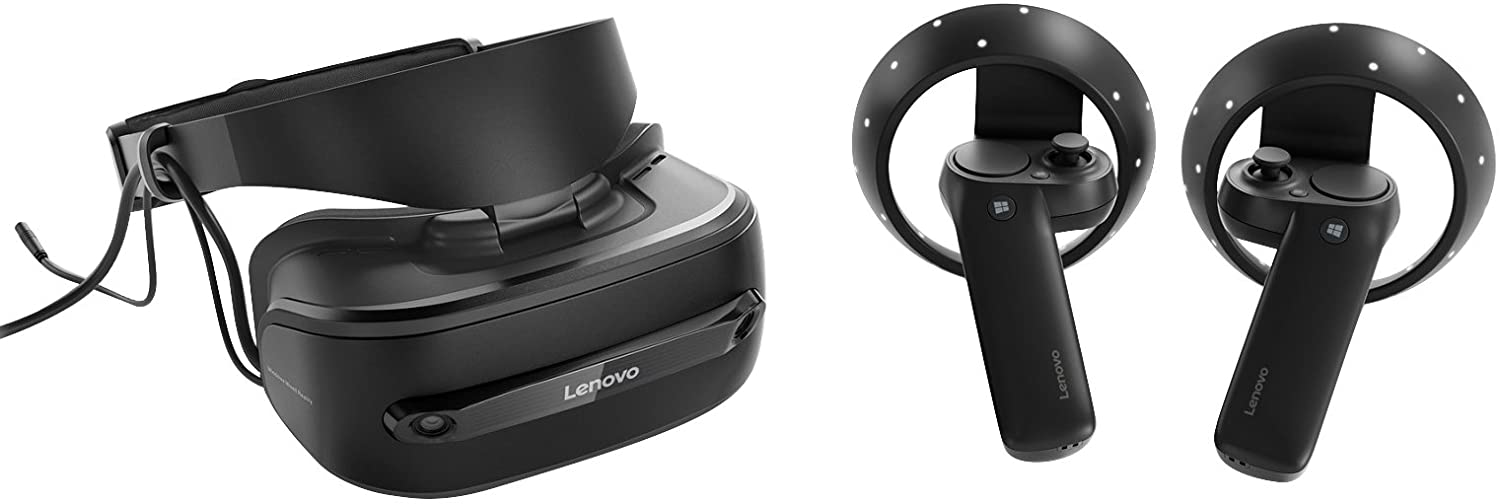
\includegraphics[scale=0.2]{Images/Estado del arte/lenovoexplorer.jpg}
    \caption[Lenovo Explore]{\textit{Lenovo Explore}r\footnotemark.}
    \label{fig:lenovoExplorer}
\end{figure}

\footnotetext{Fuente: \href{https://www.lenovo.com/es/es/smart-devices/virtual-reality/lenovo-explorer/Lenovo-Explorer/p/G10NREAG0A2}{\nolinkurl{https://www.lenovo.com/Lenovo-Explorer/p/G10NREAG0A2}}}

\parindent=0em
\subsection{Comparación de dispositivos}
\noindent


\parindent=0em
\section{Usos}
\noindent

La realidad mixta está ganando importancia frente a la realidad virtual y la realidad aumentada, ya que utiliza lo bueno de las dos tecnologías, lo cual provoca que se utilice a día de hoy en diversos sectores recogidos en este apartado.

\parindent=0em
\subsection{Educación y formación}
\noindent

%https://www.microsoft.com/es-es/education/mixed-reality
Las tecnologías inmersivas hacen una gran aportación a la educación en forma de motivación y, una manera innovadora de aprender para los estudiantes. Alice Bonasio~\cite{microsoftEducation} afirma que la realidad mixta ofrece beneficios en la educación en el proceso cognitivo, sirve como acogida social, mejora el aprendizaje emocional y permite un cambio de comportamiento en los aprendices.\\ 

Por un lado, la realidad mixta ofrece un entorno seguro para practicar y perfeccionar habilidades y reduce el cuello de botella debido al exceso de información generando un mayor razonamiento abstracto y pensamiento crítico.\\ 

Por otra parte, al aumentar el uso de estas tecnologías en instituciones educativas se está brindando su uso a personas que anteriormente no tenían acceso a ellas, asimismo, al permitir experiencias colaborativas entre usuarios se mejoran las relaciones sociales de los usuarios.\\

Las simulaciones permiten a los usuarios practicar situaciones rutinarias o acceder a experiencias que serían inalcanzables en el mundo real. Los estudiantes que aprenden a través de la realidad mixta presentan un mayor nivel de concienciación con el entorno, además, gracias a la realidad mixta se puede realizar una formación de empleados más eficiente.\\

Muchos tipos de formaciones pueden ser remplazadas por un entorno en realidad mixta de situaciones reales o instrucciones con el mundo real frente a los empleados, lo cual hace que al enfrentarse a estas situaciones reales (no como lo harían sin esta tecnología, solo con casos teóricos) ganen aptitudes de una manera más rápida.\\
 
En conclusión, la realidad mixta en el ámbito de la educación reduce la carga cognitiva, aumenta la retención de conocimientos y desencadena la empatía~\cite{microsoftEducation}.\\

%https://www.microsoft.com/es-es/p/vr-frog-dissection-ribbit-ing-discoveries/9mvjk426cbt1?CustomerIntent=Consumer&activetab=pivot%3Aoverviewtab#


Desde la perspectiva de las aplicaciones, se pueden encontrar alguna de ellas como por ejemplo,\textit{VR Frog Dissection: Ribbit-ing Discoveries} (figura \ref{fig:vrfrogdissectioncapturas}) una experiencia de realidad mixta a través de la cual los usuarios pueden aprender cómo se disecciona una rana.

\begin{figure}[htbp]
\centering
    \hspace{-4mm}
    \begin{minipage}{0.5\textwidth}
        \centering
        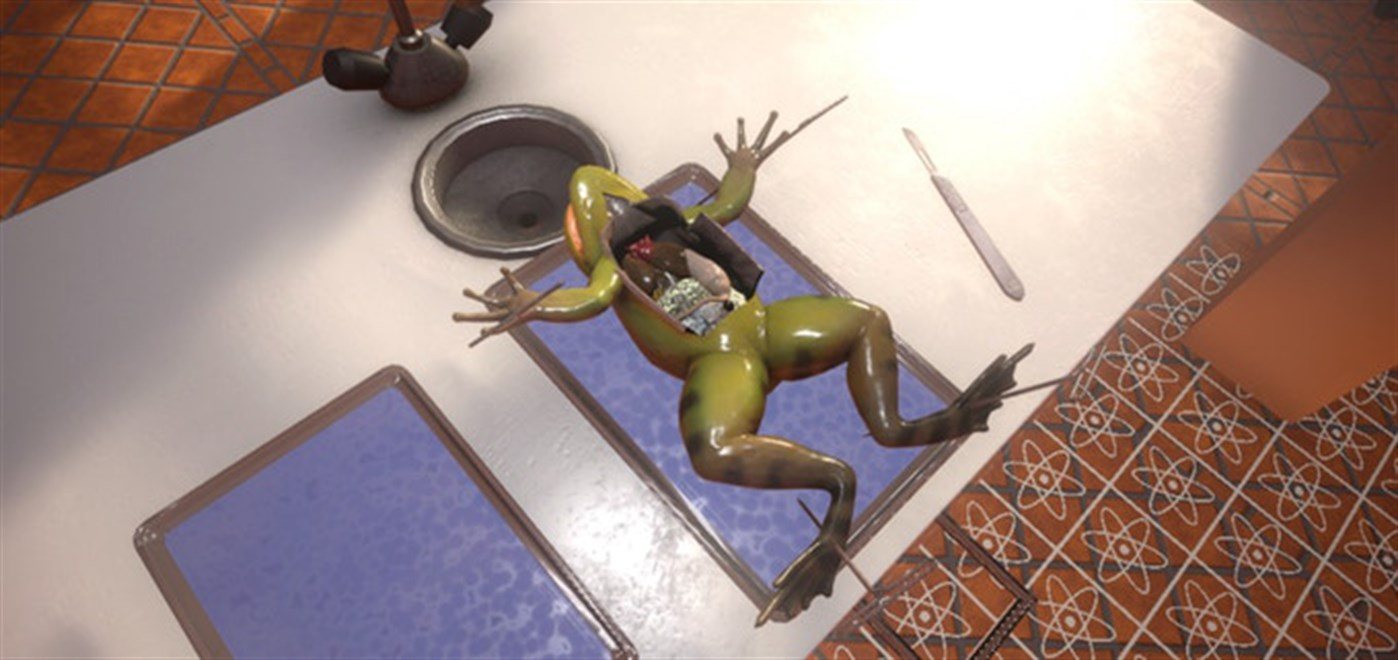
\includegraphics[scale=0.16]{Images/Estado del arte/frogDisection1.jpeg}\\
    \end{minipage}
    \begin{minipage}{0.5\textwidth}
        \centering
        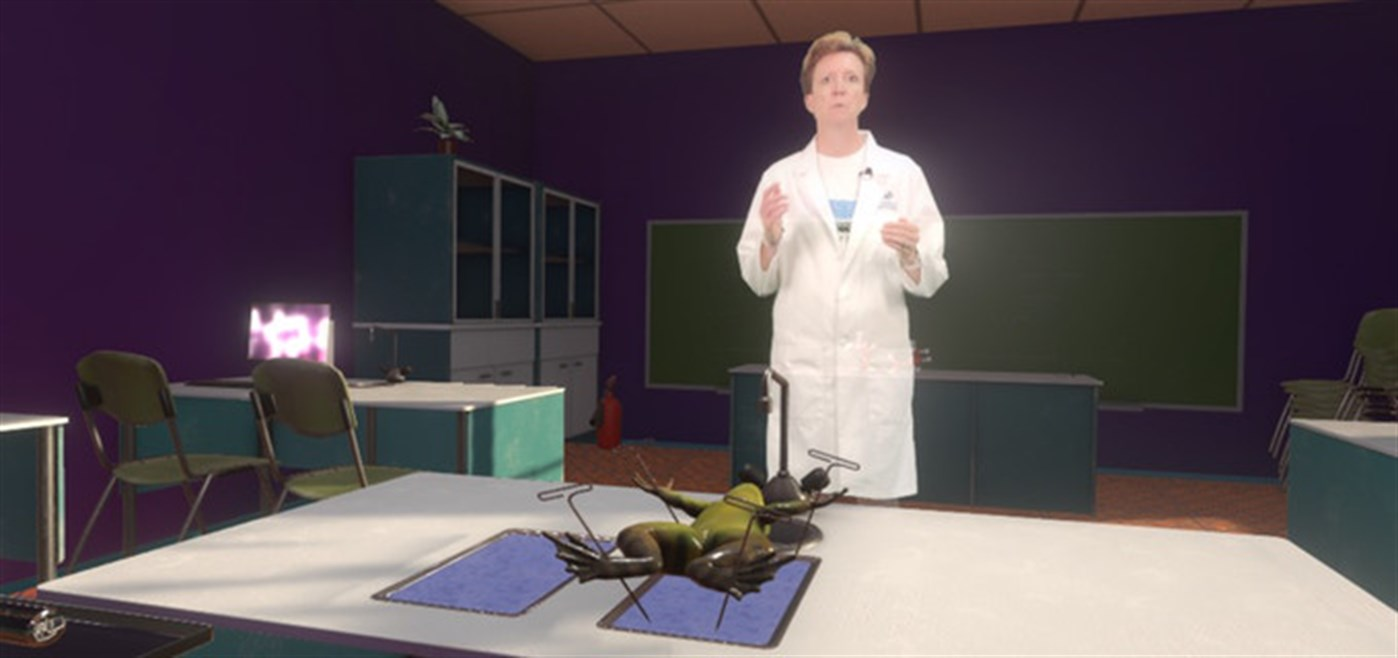
\includegraphics[scale=0.16]{Images/Estado del arte/frogDisection2.jpeg}\\
    \end{minipage}\\
    \caption[VR Frog Dissection: Ribbit-ing Discoveries]{\textit{VR Frog Dissection: Ribbit-ing Discoveries}\footnotemark.}
    \label{fig:vrfrogdissectioncapturas}
\end{figure}

\footnotetext{VR Frog Dissection: Ribbit-ing Discoveries: \href{https://www.microsoft.com/es-es/p/vr-frog-dissection-ribbit-ing-discoveries/9mvjk426cbt1?CustomerIntent=Consumer&activetab=pivot\%3Aoverviewtab#}{\nolinkurl{https://www.microsoft.com/es-es/p/vr-frog-dissection}}}

Otras de las muchas experiencias que nos ofrece la plataforma \textit{Windows Mixed Reality} son \textit{HoloTour} (una combinación de vídeo de 360 grados, sonido espacial y paisajes holográficos) o la aplicación de navegación 3D a través del cuerpo humano llamada \textit{Holo-Human}. Se puede usar esta experiencia de forma colaborativa para descubrir la anatomía de un cuerpo humano (figura \ref{fig:capturaHoloHuman}).

\begin{figure}[H]
    \centering
    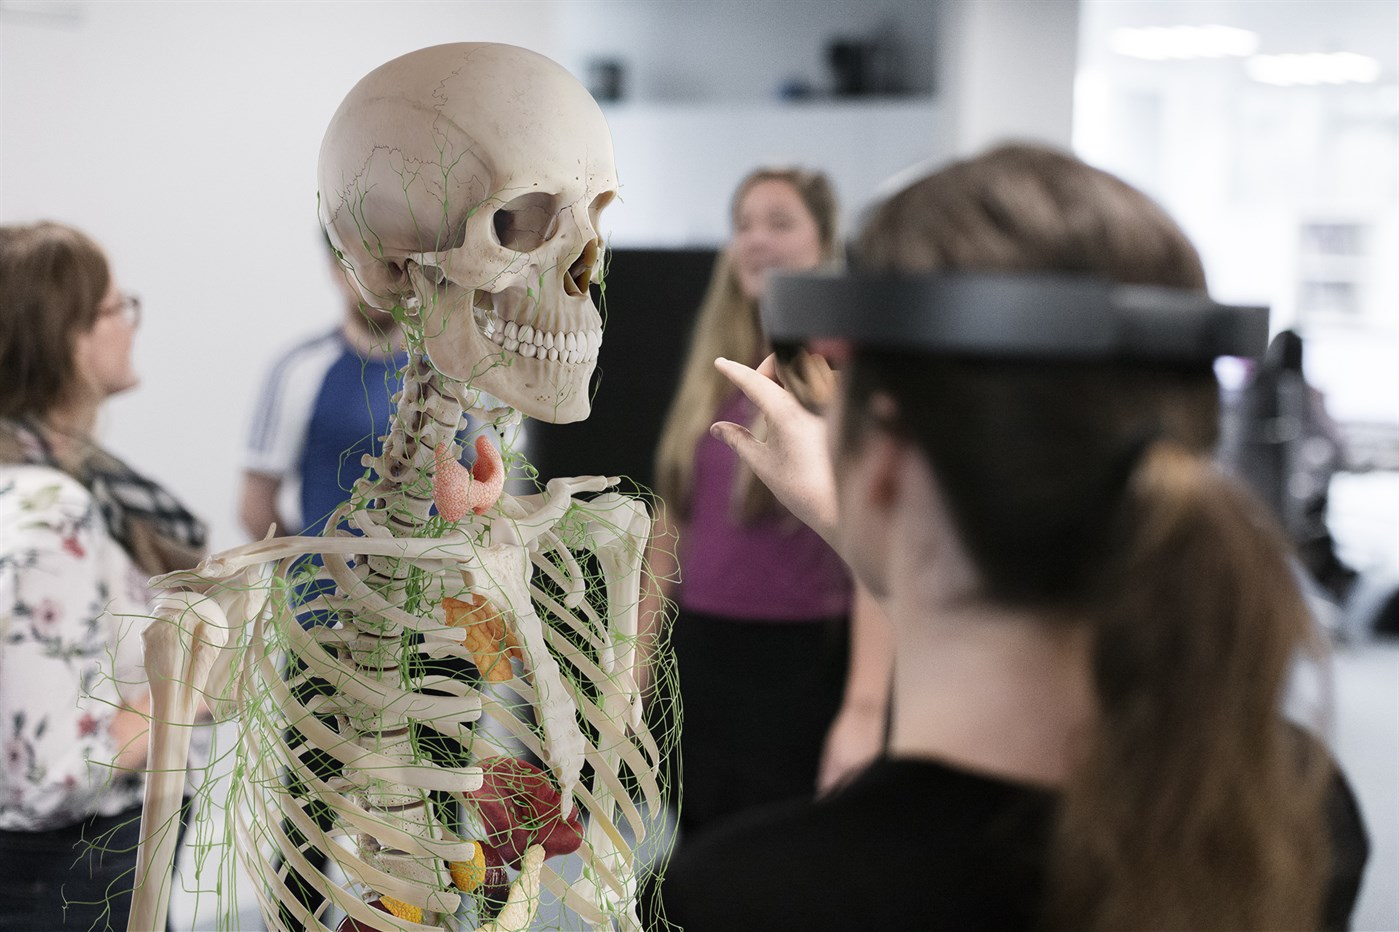
\includegraphics[scale=0.18]{Images/Estado del arte/holohuman.jpeg}
    \caption[Uso de la aplicación \textit{Holo-Human}]{Uso de la aplicación \textit{Holo-Human}\footnotemark.}
    \label{fig:capturaHoloHuman}
\end{figure}

\footnotetext{\textit{Holo-Human}: \href{https://www.microsoft.com/es-es/p/holo-human/9pggbknrbckj?CustomerIntent=Consumer&activetab=pivot\%3Aoverviewtab#}{\nolinkurl{https://www.microsoft.com/es-es/p/holo-human}}}

%https://www.microsoft.com/es-es/p/holo-human/9pggbknrbckj?CustomerIntent=Consumer&activetab=pivot%3Aoverviewtab#


\parindent=0em
\subsection{Industria}
\noindent

%https://news.microsoft.com/es-es/2019/06/18/airbus-vuela-mas-alto-con-ayuda-de-la-tecnologia-de-realidad-mixta-de-microsoft/

%https://marquesme.com/5-beneficios-clave-de-realidad-mixta-para-la-industria/

%https://www.abc.es/tecnologia/informatica/soluciones/abci-realidad-mixta-y-hologramas-llegan-reuniones-trabajo-sector-inmobiliario-201903170153_noticia.html

Otro ámbito que es potenciado por la realidad mixta es la industria, esta tecnología beneficia a este sector de las siguientes formas:

\begin{itemize}
    \item \textbf{Proceso de control de calidad más rápido:} Estos largos procesos de control de calidad se ven reducidos notablemente haciendo uso de imágenes, textos o modelos 3D. Esto da lugar a ensamblajes más rápidos y con menos errores.
    
     \item \textbf{Mantenimientos más rápidos:} Se pueden sustituir manuales de reparación tediosos por simples instrucciones en el entorno de realidad mixta. Otro uso para agilizar el mantenimiento es el que hace, por ejemplo, la empresa de ascensores \textit{ThyssenKrupp}. En ella, sus empleados hacen uso de estos cascos de realidad mixta para realizar llamadas al soporte técnico que les guía con facilidad gracias a poder superponer en tiempo real distintos elementos del ascensor a través de la retransmisión que ofrecen las gafas.
     
     \item \textbf{Reuniones colaborativas:} Los cascos de realidad mixta aportan utilidad de cara a trabajar de forma colaborativa mediante reuniones a distancia en tiempo real. Se crean hologramas de los participantes en un entorno concreto en el que pueden colaborar en diversos proyectos o participar de forma conjunta en lluvias de ideas.
     
\end{itemize}

 Todos los puntos anteriores fomentan el crecimiento de la empresa en forma de automatizar procesos, minimizar tiempos y reducir costes, es por esto que el uso de dicha tecnología es necesaria para ser competitivos.\\

La empresa de diseño, fabricación y venta de aviones civiles Airbus es una de las beneficiadas por la realidad mixta, esta empresa afirma que el uso de gafas de realidad mixta en su producción aumenta su productividad y su eficacia, además, utiliza estos HMD para formar a sus empleados (figura~\ref{fig:ingenierosAirbusHololens2}). Del mismo modo, aseguran que la tecnología \textit{hand tracking} de algunas de las gafas aporta seguridad a los empleados gracias a tener las manos libres. \\

\begin{figure}[h]
    \centering
    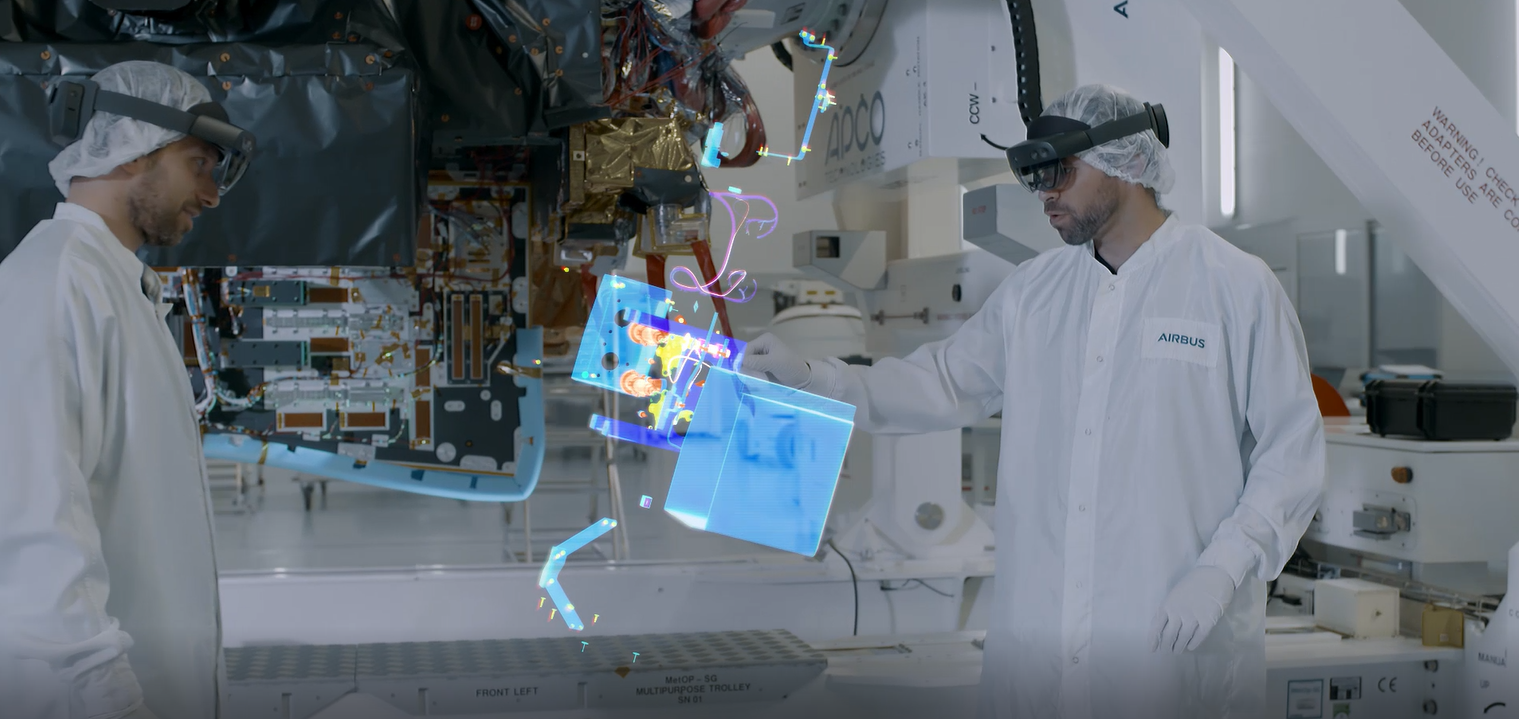
\includegraphics[scale=0.3]{Images/Estado del arte/ingenierosAirbus.png}
    \caption[Diseñadores de Airbus haciendo uso de la realidad mixta]{Diseñadores de Airbus haciendo uso de la realidad mixta\footnotemark.}
    \label{fig:ingenierosAirbusHololens2}
\end{figure}

\footnotetext{Fuente: \href{https://news.microsoft.com/es-es/2019/06/18/airbus-vuela-mas-alto-con-ayuda-de-la-tecnologia-de-realidad-mixta-de-microsoft/}{\nolinkurl{https://news.microsoft.com/es-es/2019/06/18/}}}

Por último, otro uso industrial de la realidad mixta es el que se puede aplicar al diseño de apariencia y estética de productos industriales como coches o motocicletas~\cite{mrinaesthethics}. En este caso, la aplicación \textit{Spacedesign} sustituye las técnicas de prototipado rápido por una experiencia de realidad mixta para realizar esos bocetos en tres dimensiones.

%\input{Sections/C3/Entretenimiento}
\parindent=0em
\subsection{Atención médica}
\noindent

%https://blogs.windows.com/windowsexperience/2018/03/08/how-mixed-reality-is-changing-the-game-for-healthcare-from-performing-live-surgeries-to-delivering-ultrasounds-in-3d/

Existen diversos usos de la realidad mixta en la atención médica, en primer lugar, la empresa \textit{CAE Healthcare} es una de las líderes en simulaciones tecnológicas y en recursos para mejorar el desempeño en las clínicas. \textit{CAE VimedixAR} es un simulador de ultrasonido diseñado por dicha empresa para las \textit{HoloLens}, de esta forma, los profesionales pueden manipular partes anatómicas (rotándolas y escalándolas).\\

Otra aplicación diseñada por esta empresa es \textit{CAE Lucina} (figura \ref{fig:caelucina}). Se trata de un simulador de partos donde los profesionales pueden realizar la extracción completa del feto en cualquier situación excepcional (estando así preparados para cualquier imprevisto).

\begin{figure}[h]
    \centering
    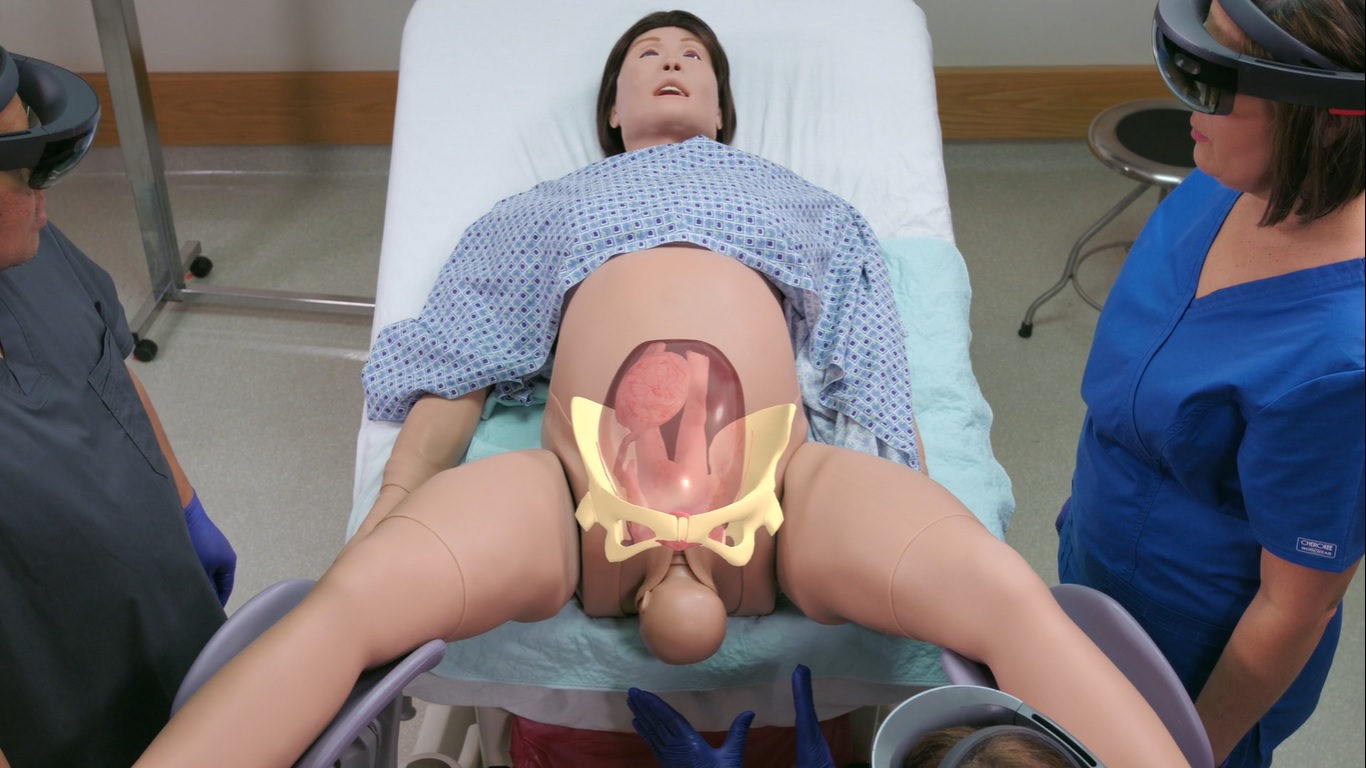
\includegraphics[scale=0.38]{Images/Estado del arte/caehealthcareparto.jpg}
    \caption{CAE Lucina en ejecución con las HoloLens.}
    \label{fig:caelucina}
\end{figure}

Por otro lado, la empresa \textit{Pearson} ha desarrollado una aplicación llamada \textit{HoloPatient} la cual sirve para formar estudiantes de enfermería. El programa se basa en una experiencia que permite aprender sin necesidad de actores o pacientes que se necesitarían sin usar esta tecnología. \textit{HoloPatient} salió al mercado en Abril del año 2018.\\

Existen otros proyectos como el que viene de la mano de \textit{SphereGen} en colaboración con una universidad, bautizado con el nombre de \textit{Learning Heart} (figura \ref{fig:learningheartspheregen}). Esta aplicación enfocada a su uso a través de las \textit{HoloLens}, permite a sus usuarios aprender sobre el corazón (de manera individual o colaborativa) viéndolo desde cualquier ángulo y posición. 

\begin{figure}[h]
    \centering
    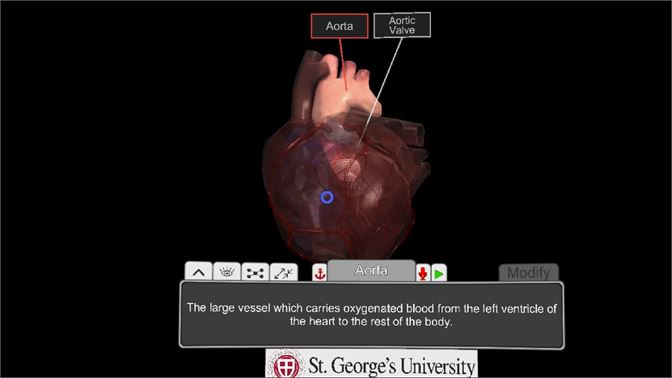
\includegraphics[scale=0.65]{Images/Estado del arte/learningheartspheregen.jpeg}
    \caption{\textit{Learning Heart} en ejecución.}
    \label{fig:learningheartspheregen}
\end{figure}


%Foto del learning 
%https://www.microsoft.com/en-us/p/learning-heart/9pghzvfwxpmb?activetab=pivot:overviewtab}


En cuanto a la radiología, \textit{DICOM Director} aporta una gran ayuda a estos expertos permitiéndoles ver y analizar todo tipo de escaneos en 3D. Los radiólogos y doctores pueden ver estas radiografías haciendo uso de sus \textit{HoloLens} o sus cascos de realidad mixta de Windows, igualmente, la aplicación genera un modelo 3D de esas imágenes (figura \ref{fig:dicomDirector}) los cuales se pueden rotar y analizar. De esta manera, \textit{DICOM Director} se utiliza también como herramienta de comunicación entre doctores para compartir estos modelos.

\begin{figure}[h]
    \centering
    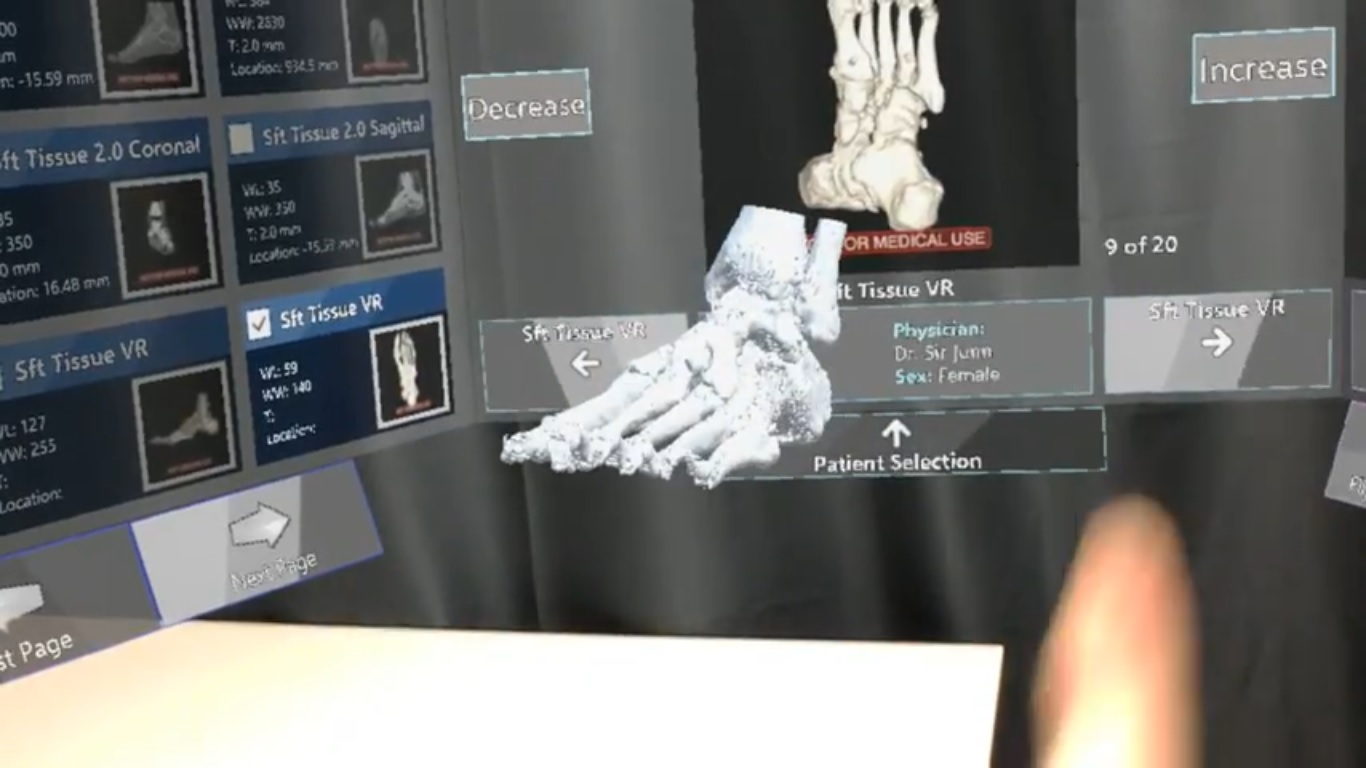
\includegraphics[scale=0.25]{Images/Estado del arte/dicomdirector.jpg}
    \caption{Usuario rotando el modelo 3D de una radiografía en\textit{DICOM Director}.}
    \label{fig:dicomDirector}
\end{figure}

Para finalizar, la empresa \textit{Visual 3D Medical Science and Technology Development CO. LLC} ha desarrollado un producto que ha sido usado en China para realizar 200 operaciones (de rodilla, cadera y espina) gracias a la realidad mixta. Incluso se está utilizando para preparar a los cirujanos antes de entrar a la sala de operaciones, reproduciendo la operación a través de las gafas. 








\parindent=0em
\section{APIs}
\noindent
A la hora de generar experiencias de realidad mixta existen diversas APIs (del inglés \textit{ApplicationProgramming Interface}) que pese a no estar enfocadas en crear entornos de realidad mixta, pueden ser utilizadas para ello.\\

En esta sección se tratan dos APIs destacables a la hora de generar dichos entornos: ARcore y Vuforia.

\parindent=0em
\subsection{ARCore}
\noindent

ARCore es un kit de desarrollo de Google \cite{ARCoreOverview} enfocado a construir experiencias de realidad aumentada en dispositivos Android. Tiene distintas APIs que permiten utilizar el teléfono para entender el mundo real e interactuar con él. ARCore utiliza tres pilares fundamentales para integrar el contenido virtual en el mundo físico:

\begin{enumerate}[label=\arabic*)]
    \item \textbf{\textit{Motion tracking}:} ARCore utiliza unos \textbf{puntos característicos} como elementos de referencia para detectar si se produce un cambio en la posición. Esta información se combina con los datos de la velocidad, orientación y fuerzas gravitacionales del aparato para estimar la posición y orientación de la cámara.
    
     \item \textbf{\textit{Environmental understanding}:} Esta tecnología utiliza concentraciones de estos puntos característicos mencionados anteriormente uniéndolos de manera horizontal o vertical para formar planos. Esta información se puede utilizar para colocar elementos en superficies lisas.
     
     \item \textbf{\textit{Light estimation}:} Para poder dar una iluminación a nuestros objetos virtuales acorde al mundo real, la plataforma detecta la información de la luz del entorno y realiza una estimación de la intensidad y el color.
\end{enumerate}

A la hora de colocar un elemento virtual en el mundo físico, cuando el usuario interactúa con la pantalla en un punto concreto, ARCore comprueba si existe algún plano o punto característico en ese punto y coloca el objeto ahí utilizando un \textbf{ancla} (posiciones en el mundo físico para mantener el control de los objetos en el tiempo).\\

Por ejemplo, si colocamos un cubo en una puerta y nos desplazamos, al volver a apuntar a la puerta podremos ver que el cubo sigue ahí (gracias a los anclas). No solo se pueden utilizar estos anclas en un mismo dispositivo, sino que ARCore ofrece la \textit{ARCore Cloud Anchor API} mediante la cual se guarda la posición de los anclas en la nube, de tal forma que varios móviles pueden observar el mismo objeto virtual colocado por una persona. Esto permite compartir los entornos con varios usuarios simultáneamente.\\

%https://developers.googleblog.com/2019/12/blending-realities-with-arcore-depth-api.html

Recientemente ARCore ha introducido la \textit{ARCore Depth API} lo cual supone un gran avance a la hora de calcular profundidades en el mundo virtual ya que funciona con una única cámara (antes se requerían dispositivos con grandes capacidades hardware). La profundidad es calculada mediante un algoritmo que toma múltiples fotos de distintos ángulos y estima la distancia a cada píxel. Esto permite a los desarrolladores crear mapas de profundidad para generar un efecto de oclusión (sección~\ref{sec:oclusion}).\\

Aunque esta API no es dependiente de cámaras o sensores específicos, la experiencia mejorará notablemente al utilizar dispositivos con un mejor hardware como sensores ToF (sensores que miden la profundidad en función a la distancia que tarda la emisión y recepción de un haz de luz infrarrojo) dado que permitirá activar la funcionalidad de la oclusión dinámica, es decir, poder hacer el efecto de oclusión con objetos en movimiento.\\

Actualmente ARCore se puede utilizar en la plataforma de desarrollo Unity, en Unreal Engine o a través del entorno de desarrollo integrado Android Studio. Aunque ARCore es gratuito, no está soportado por todos los dispositivos móviles o tabletas, existe una lista de dispositivos soportados\footnotemark.\\

\footnotetext{Dispositivos que soportan ARCore: \href{https://developers.google.com/ar/discover/supported-devices
}{\nolinkurl{https://developers.google.com/ar/discover/supported-devices}}}

Si se quiere desarrollar algo para iOS, la alternativa a ARCore se llama ARKit~\cite{arKitIntro}. Este kit de desarrollo de Apple ofrece opciones muy similares a ARCore como detección del entorno, cálculo de la profundidad o sesiones colaborativas, todo para dispositivos con iOS.




\parindent=0em
\subsection{Vuforia}
\noindent

Vuforia Engine~\cite{vuforiaMain} es una plataforma enfocada al desarrollo de aplicaciones de realidad aumentada, se puede utilizar en todos los dispositivos móviles y tablets, además, permite a los desarrolladores añadir funcionalidades de visión por computador. Con Vuforia se pueden crear aplicaciones para dispositivos Android, iOS y para dispositivos Windows. \\

Esta librería ofrece las siguientes herramientas: 

\begin{itemize}
    \item \textit{\textbf{Area Target Generator}}: Aplicación de escritorio que toma como entrada el escáner de un modelo 3D del entorno y genera un \textit{area target} (en el ámbito de Vuforia se refiere a un entorno donde se controla el \textit{tracking} de objetos y se permite colocar elementos).
    
    \item \textit{\textbf{Area Targets Test App}}: Se trata de una aplicación para poder comprobar la calidad del \textit{area target} generado al hacer el escáner de forma rápida, es decir, un área de pruebas de entornos 3D generados.
    
    \item \textit{\textbf{Model Target Generator}}: El \textit{Model Target Generator} es otra aplicación de escritorio mediante la cual se puede generar un \textit{area target} tomando como entrada un modelo 3D ya existente (en lugar de realizar un escáner). Esta aplicación soporta extensiones de archivo como \textit{.obj}, \textit{.fbx} o \textit{.stl} entre otros.
    
    \item \textit{\textbf{Model Target Test Application}}: En este caso se trata de una aplicación para móviles Android que se utiliza para evaluar \textit{model targets} (modelos que se utilizan para reconocer y hacer el \textit{tracking} de determinados elementos del mundo real gracias a su forma).
    
    \item \textit{\textbf{Vuforia Object Scanner}}: Aplicación de Android que se utiliza para escanear elementos del mundo real y generar archivos compatibles con Vuforia para definir un \textit{model target}.
    
    \item \textit{\textbf{Target Manager}}: Herramienta web que permite al desarrollador crear y manipular sus \textit{targets}.
\end{itemize}

Respecto al \textit{tracking}, Vuforia calcula la posición del usuario en función de detalles en el entorno tomados por la cámara (como los puntos característicos de ARCore), asimismo, utiliza la Unidad de Medición Inercial para controlar los 6DoF del dispositivo.\\

A diferencia de ARCore, para utilizar este kit de desarrollo es necesario pagar alguno de sus planes. 

\parindent=0em
\section*{Resumen}
\noindent

En este capítulo se han tratado los conceptos de las tres realidades que abarcan las XR. Dichos conceptos han servido para poder distinguir las distintas realidades entre ellas, además, se han contado las tecnologías que hacen falta para sus usos. Dentro de estas tecnologías cabe destacar la importancia del \textit{tracking} a través de distintas técnicas.\\

Una vez conocidos lo componentes necesarios para su funcionamiento se puede hablar de los distintos dispositivos que permiten su uso, desde teléfonos móviles hasta HMDs donde se ha podido ver que estos tienen distintos tipos de conectividad, pueden utilizar mandos o no e incluso estar dotados de tecnología \textit{eye tracking}.

Por último, la realidad mixta potencia distintos campos como la educación, la atención médica, la industria o los videojuegos. Para poder desarrollar aplicaciones de realidad aumentada y realidad mixta destacan distintas APIs como ARCore, ARKit o Vuforia.

En este capítulo se ha visto el funcionamiento de las XR y sus usos. En el siguiente capítulo se podrán ver distintas aplicaciones haciendo uso de la API ARcore para conseguir un efecto de oclusión.



\parindent=0em
\chapter{Oclusión en tiempo real con Arcore y Unity}
\noindent

%Oclusión en tiempo real con Arcore y Unity
    %Integracion de arcore con unity
    %Nube de puntos ARcore
    %Shader de profundidad
    %Shader de oclusión
    %Optimización
    %Resumen y problemas de Arcore en Unity

\parindent=0em
\section{Integración de ARCore con Unity}
\noindent

La integración de ARCore en Unity se realiaza mediante los llamadaos packages (paquetes) de Unity. 
Dependiendo del tipo de efecto que queramos generar dentro de nuestra aplicación tendremos que dar uso de uno u otro por las diversas características que presentan.

Evidentemente tenemos que descargar primero la SDK de ArCore de para Unity.

Para nuestro caso, necesitamos la nube de puntos proporcionada por ARCore y explicada en el siguiente apartado, por lo que descargaremos e importaremos los paquetes ArCore, XR Legacy Input y multiplayer HLAPI. Dentro de las opciones de Build de Unity, establecemos la plataforma por defecto la de Android y añadimos la escena que queramos dentro de nuestra aplicación. En PlayerSettings, tenemos que quitar el tipo de renderizado Vulkan y añadir .NET 4X, así como establecer el mínimo Api Level a 24. Finalmente, habilitar ARCore supported dentro de PlayerSettings -> XRSettings.

\parindent=0em
\section{Nube de puntos}
\label{sec:nubeDePuntos}
\noindent

\parindent=0em
\subsection{Definición}
\noindent

La definición de nube de puntos depende del ámbito en la que esta se aplique. Es por ello, que encontramos varias definiciones ~\cite{DefinicionesNubePuntos1} ~\cite{DefinicionesNubePuntos2} ~\cite{DefinicionesNubePuntos3} dentro de incluso un mismo proyecto para esta. Sin embargo, todas coinciden en el mismo aspecto, y es que \textit{ una nube de puntos es un producto resultante del escaneo láser o por fotogrametría (en tiempo real o en diferido). Este está expresado por millones de puntos posicionados tridimensional mente en el espacio (con coordenadas X, Y, Z) formando una entidad física y destinados a representar virtualmente la superficie externa de esta}. Esta nube de puntos, además de contener la información de posiciones de los mismos también puede contener información añadida como el color de cada punto, su reflexión o la iluminación que recibe, o el tamaño del mismo.\\
\parindent=0em
\subsection{Generación}
\noindent

Como en la definición se ha comentado, existen varias maneras de generar una nube de puntos en la actualidad (escaneo láser, fotogrametría o sensores de luz infrarroja ToF). Pese a todas estas formas de generación de nubes de puntos, en este caso se profundizará en la llamada \textit{Structure for motion}, que entra dentro de la fotogrametría y es la forma más común de uso y la utilizada por ARCore. \\

En concreto, ARCore y ARKit (la versión de ARCore para iOS) utilizan la técnica llamada \textit{visual-inertial odometry} ~\cite{ VisualOdometry}. Este proceso telemétrico combina información del dispositivo como puede ser el giróscopo o el acelerómetro con visión analítica generada por ordenador visible a la cámara ~\cite{ WorldTracking}. \\

Este proceso es usado en una gran variedad de aplicaciones, sobre todo robóticas, como por ejemplo en la exploración de Marte con el \textit{Rovers} ~\cite{ MarsExploration}. \\

Esta tecnología, la de ARCore, utiliza la cámara del dispositivo para identificar puntos interesantes, llamados \textit{features}, y rastrea su movimiento a lo largo del tiempo. Esto último lo realiza con una combinación del movimiento de esos puntos y la lectura de los sensores de inercia del dispositivos (tanto la posición como la orientación del movimiento en el espacio).\\

Como extras dentro de estas mediciones, ARCore también detecta superficies planas y puede realizar una estimación de la iluminación del entorno. Estas capacidades combinadas son capaces de generar la nube de puntos.
~\cite{HowARCoreWorks} \\

\begin{figure}[h]
    \centering
    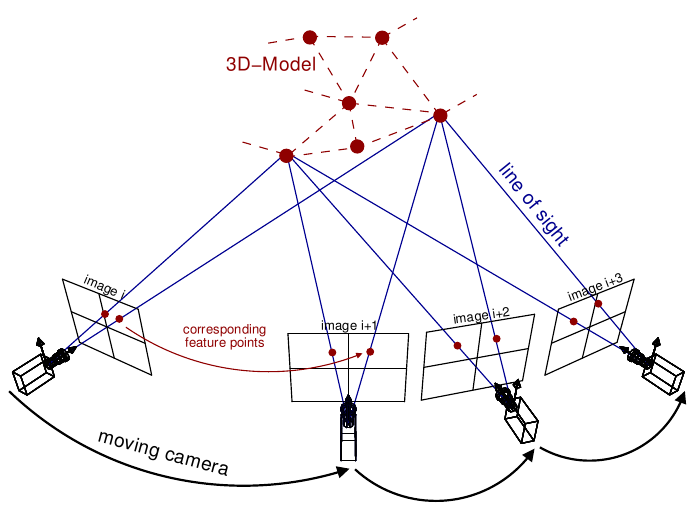
\includegraphics[scale=0.40]{Images/NubeDePuntos/StructureFromMotion(SFM).png}
    \caption[Representación de \textit{Structure From Motion (SfM)}]{Representación de \textit{Structure From Motion (SfM)}.}
    \label{fig:SFM}
\end{figure} 

Una vez comprendido a alto nivel como funciona la telemetría, ahora se profundizará un poco más dentro de este apartado.\\

Como muestra la (figura \ref{fig:Trigonometry}), se seguirán unas reglas básicas trigonométricas para resolver la posición de un único punto en el mundo real. \\

Suponiendo, por ejemplo, que se desea conocer la posición del punto A de la (figura \ref{fig:Trigonometry}), y nuestro dispositivo se encuentra en la posición B de la misma figura.
En este punto, sólo conocemos la posición y rotación de nuestro dispositivo.
Ahora realizamos un movimiento desde la posición B a la posición C. En este punto, gracias a las mediciones del dispositivo, conocemos la nueva posición y rotación (C, \textgamma), y por tanto la distancia que une a estas dos posiciones ($\overline{\mbox{#AC}}$)  que en la figura se representa por a.

Una vez se tenga tanto la posición B y C, y como sabemos la rotación del dispositivo mediante el giróscopo del mismo, tenemos los ángulos \textbeta, \textgamma. Teniendo estos dos ángulos y dado que los ángulos de cualquier triángulo han de formar 180º, también tenemos \textalpha:

$$\alpha=180º-\gamma-\beta$$

Finalmente, conocidos todos estos datos y mediante el Teorema del seno, se puede conocer tanto la distancia desde $\overline{AB}$ como $\overline{AC}$, y por consiguiente el punto A que se situará dentro de la aplicación:

$$\frac{Sen(\gamma)}{\overline{AB}}=\frac{Sen(\alpha)}{\overline{CB}} \Rightarrow \overline{AB} $$ 

$$\frac{Sen(\beta)}{\overline{AC}}=\frac{Sen(\alpha)}{\overline{CB}} \Rightarrow \overline{AC} $$ \\ \\ \\ \\

\begin{figure}[h]
    \centering
    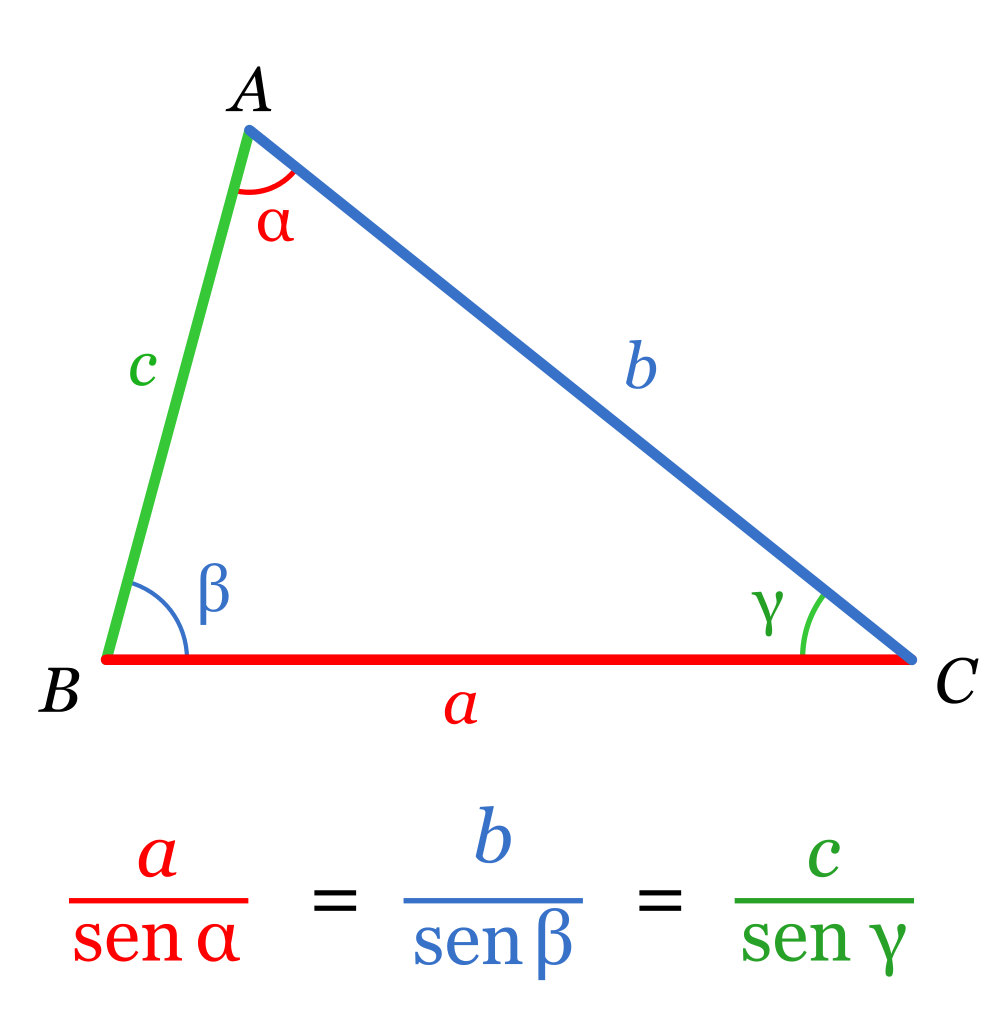
\includegraphics[scale=0.15]{Images/NubeDePuntos/Trigonometria.png}
    \caption[Principio trigonométrico para calcular distancias]{Principio trigonométrico para calcular distancias.}
    \label{fig:Trigonometry}
\end{figure}

Una vez obtengamos el punto A, sólo habrá que repetir el proceso tantas veces como \textit{``features''} haya dentro de la imagen y en consecuencia construir la nube de puntos. \\

Cuando toda la información de estos puntos esté disponible, existen varias maneras de tratarlos. Para nuestro estudio realizamos distintas pruebas aunque existen otras muchas formas de dar uso a esta nube de puntos, como la creación de una malla tridimensional para generar oclusión o simplemente obtener la información de dichos puntos para construir un objeto en tres dimensiones dentro de la aplicación.


\parindent=0em
\section{Shader de profundidad}
\noindent
\parindent=0em
\section{Shader de oclusión}
\noindent
\parindent=0em
\section{Optimización}
\noindent
\parindent=0em
\section{Resumen y problemas de ARCore en Unity}
\noindent

Pese a la publicidad de ARCore y de su tecnología, una vez comprobada esta se puede asegurar que las opciones que ofrecen están todavía muy lejos del efecto deseado y que contienen varios problemas fundamentales.\\

En varias de las imágenes mostradas por la empresa se puede apreciar como se realiza una perfecta oclusión de los objetos virtuales junto a los objetos del mundo real, incluso generando mapas de calor para conocer con total seguridad la profundidad de la escena ~\ref{fig:ARDepth}. \\

Sin embargo, tras probar toda la tecnología, sabemos que los \textit{features} mencionados en capítulos anteriores se centran en encontrar los bordes de los objetos reales para generar la nube de puntos. Pese a ello, para crear los mapas de calor o una nube de puntos óptima también sería necesario que dichas \textit{features} se generasen en superficies planas.\\

\begin{figure}[H]
    \centering
    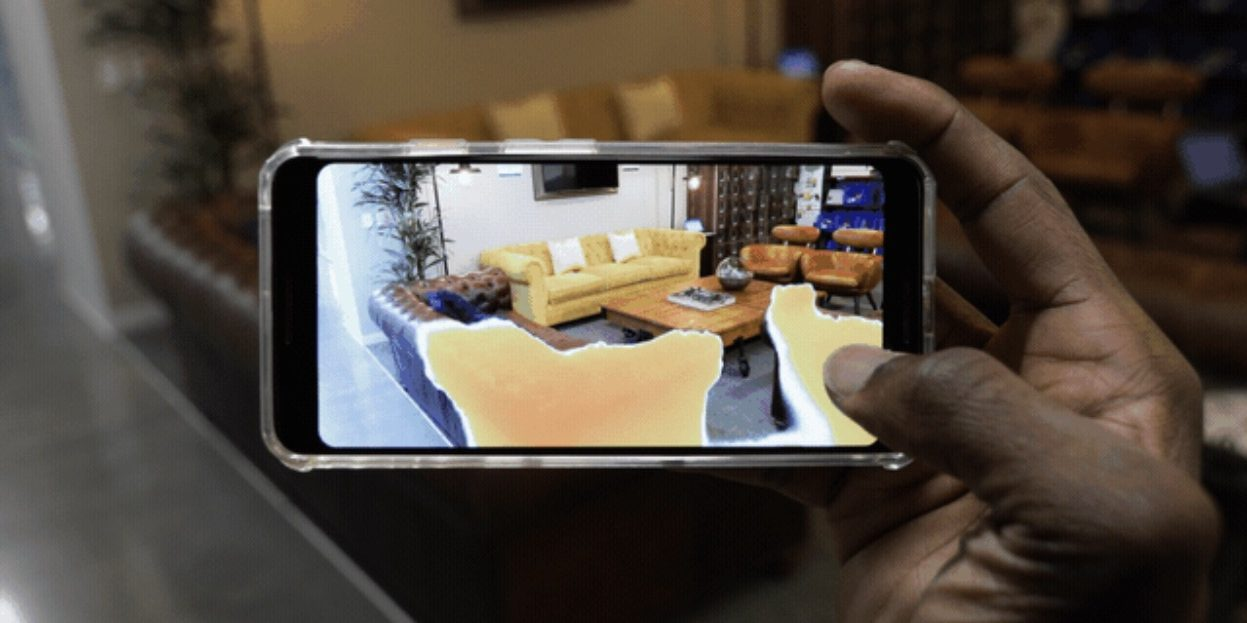
\includegraphics[scale=0.5]{Images/Optimización y resumen/ARDepth.jpg}
    \caption[Supuesto mapa de calor generado con ARCore.]{Supuesto mapa de calor generado con ARCore.}
    \label{fig:ARDepth}
\end{figure}

Pese a conocer que esta nube de puntos se genera principalmente con las \textit{features} en el contorno de los objetos, si se aumenta considerablemente el número de puntos que se pueden generar por cada frame se consigue una mejor oclusión. Esto sin embargo lleva a una caída bastante considerable del rendimiento de la aplicación así como a un consumo desmesurado de la batería del dispositivo, y por consiguiente también aumenta su temperatura.\\

A día de hoy realizar una oclusión con un nivel de detalle como el mostrado en los ejemplos de ARCore, desde un dispositivo móvil, es prácticamente imposible. Nos encontramos totalmente limitados por la tecnología de los dispositivos actuales.\\

Pese a todo esto, ARCore si que ha dado un gran paso dentro de la generación de oclusión en tiempo real. Su tecnología no precisa tener varias cámaras integradas ni sensores ToF para realizar un escaneo de la profundidad. En el futuro, cuando toda la tecnología de dispositivos móviles mejore, se podrá realizar oclusión en tiempo real sin ningún problema, aunque de momento sólo servirá para realizar fotogrametría de manera asíncrona.\\


%%%%%%%%%%%%%%%%%%%%%%%%%%%%%%%%%%%%%%%%%%%
%%%%%%%%%%%%%%%%%%%%%%%%%%%%%%%%%%%%%%%%%%% Parte 3 - Index y bibliografía
\indiceFiguras
\indiceTablas
%%%%%%%%%%%%%%%%%%%%%%%%%%%%%%%%%%%%%%%%%%%
%%%%%%%%%%%%%%%%%%%%%%%%%%%%%%%%%%%%%%%%%%% Parte 4 - BIB y licencia
\biblioTFG{16}


%%%%%%%%%%%%%%%%%%%%%%%%%%%%%%%%%%%%%%%%%%%
\end{document}